\documentclass[11pt]{article}
\usepackage{graphicx} % Required for inserting images
\usepackage{amsmath, amssymb, setspace}
\usepackage{hyperref}
\title{Some Cool Plots}
\author{Josh Sack}
\begin{document}
\maketitle 
\listoffigures
\begin{figure}
    \centering
    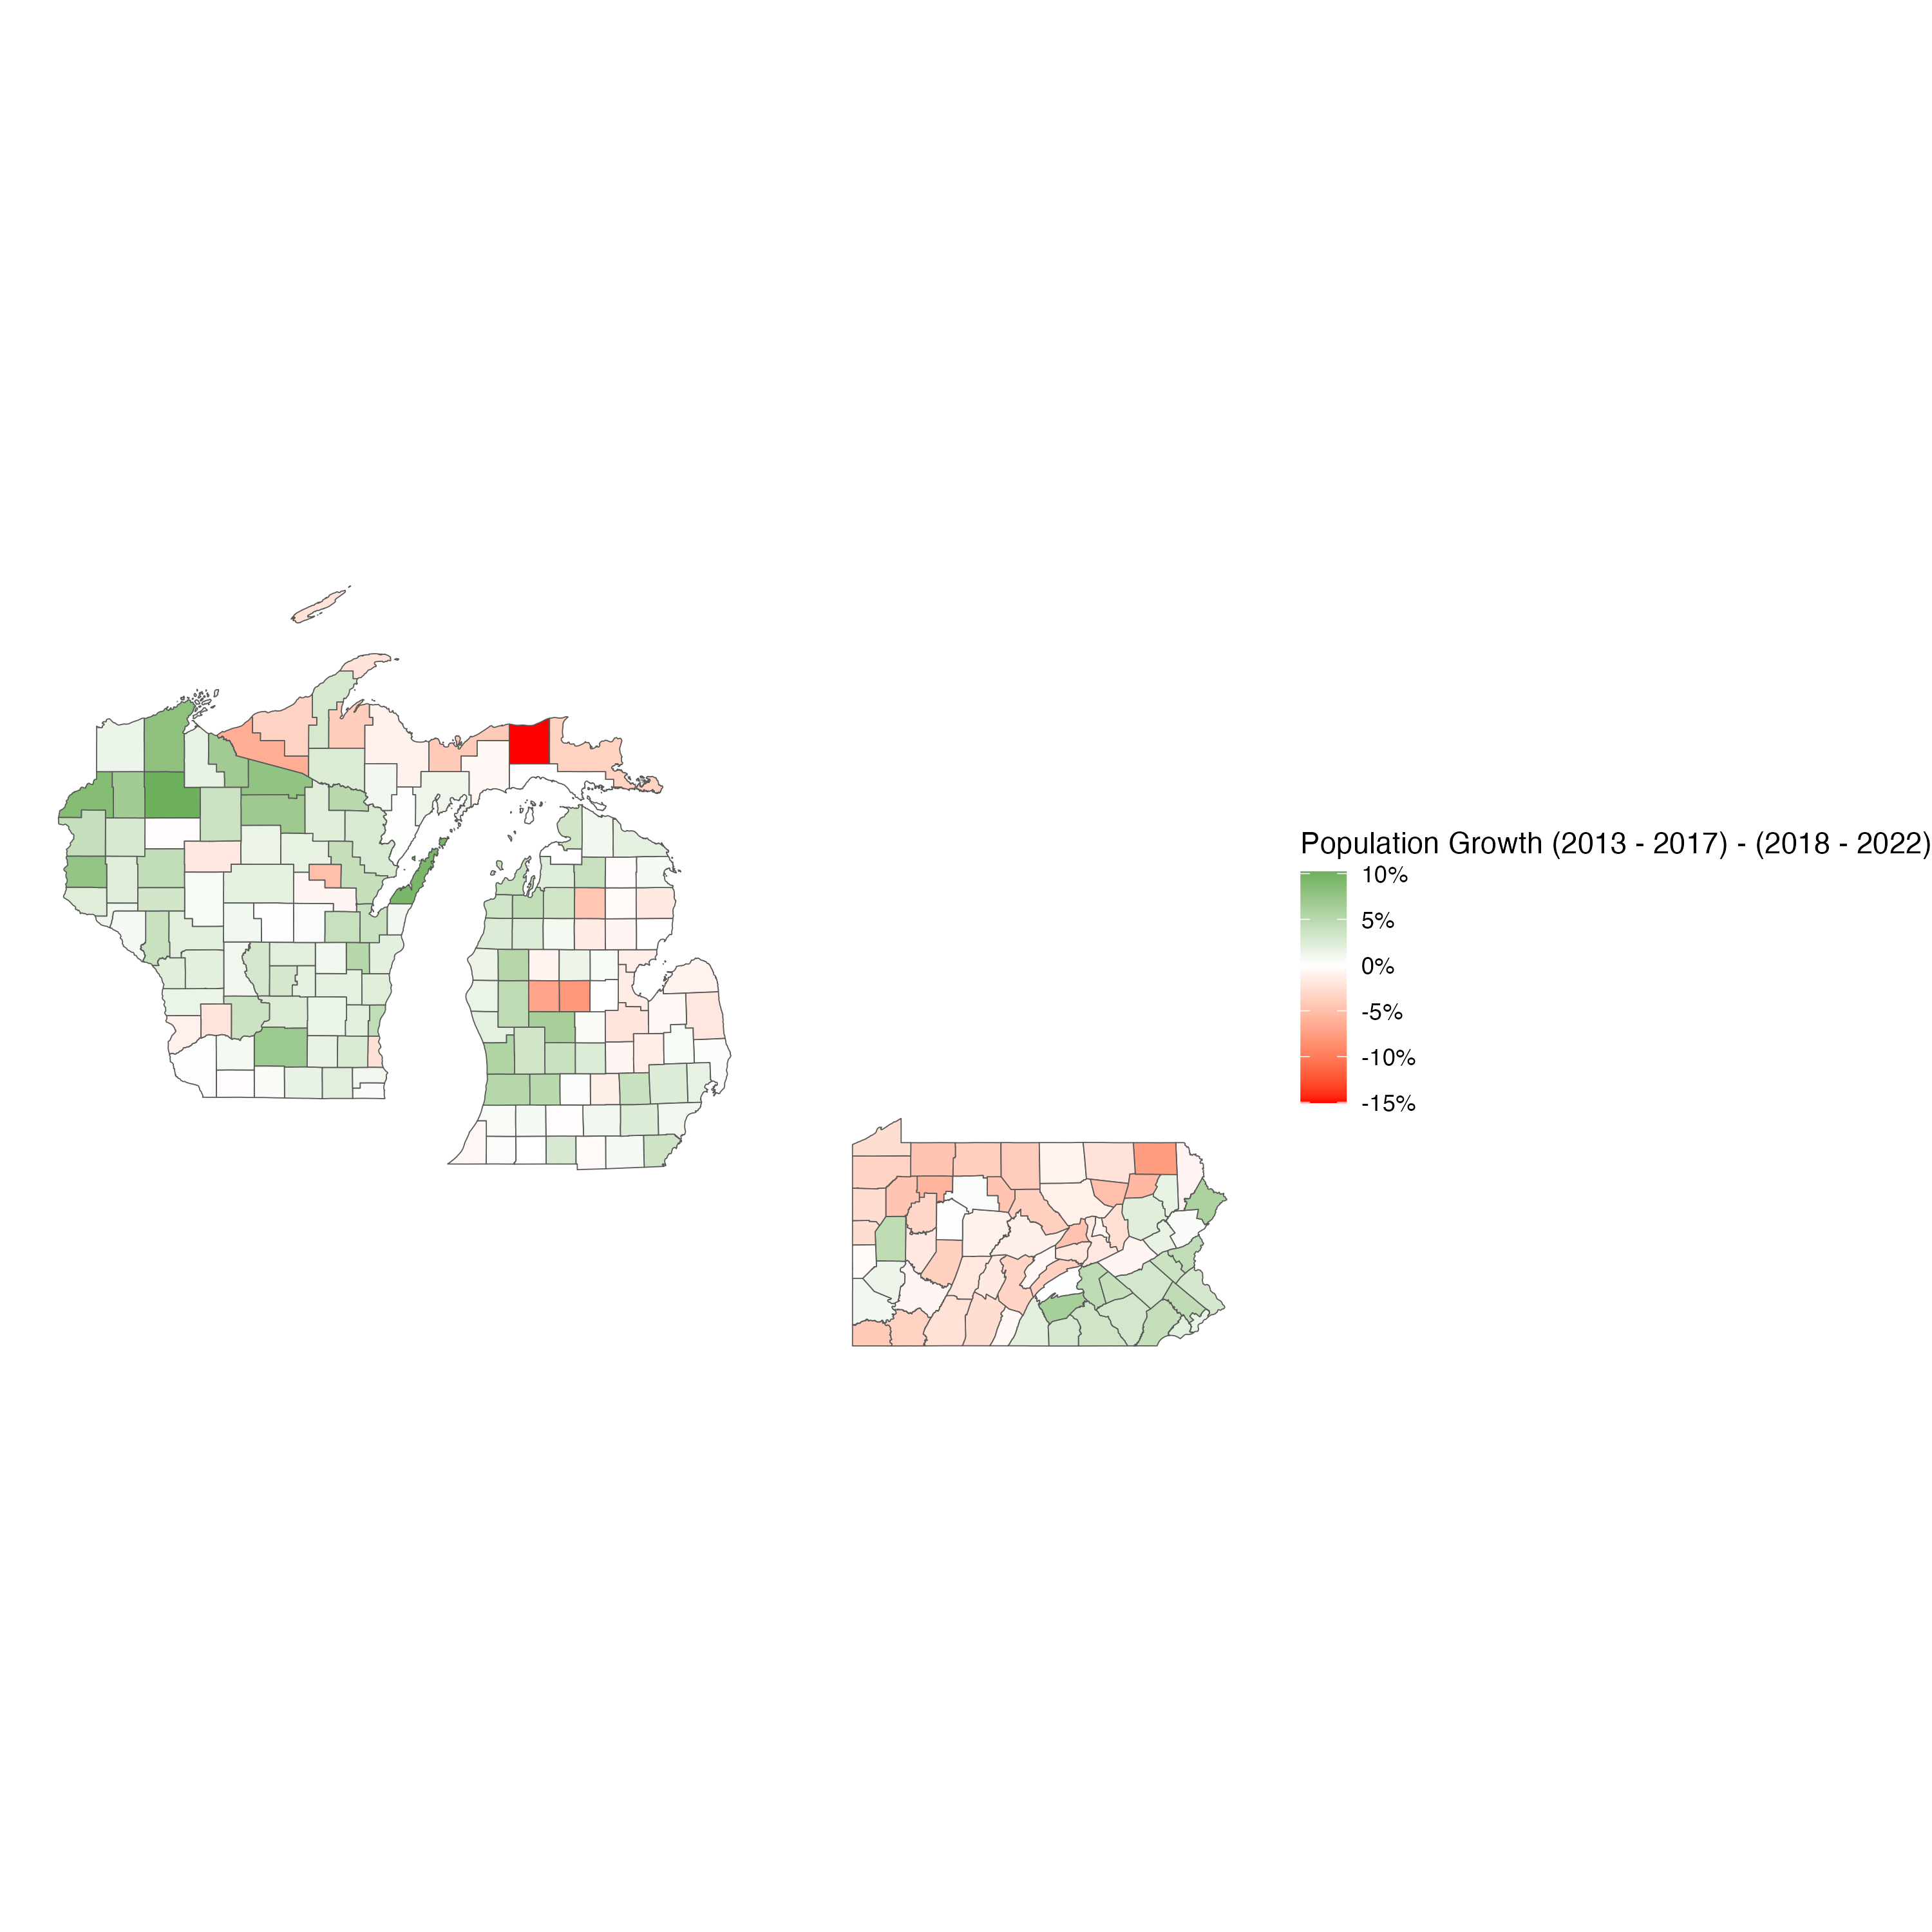
\includegraphics[width=0.9\textwidth]{plots/blue-wall-growth.png}
    \caption{The population growth rate of counties in the blue wall states from the 2017 ACS to the 2022 ACS}
\end{figure}
\begin{figure}
    \centering 
    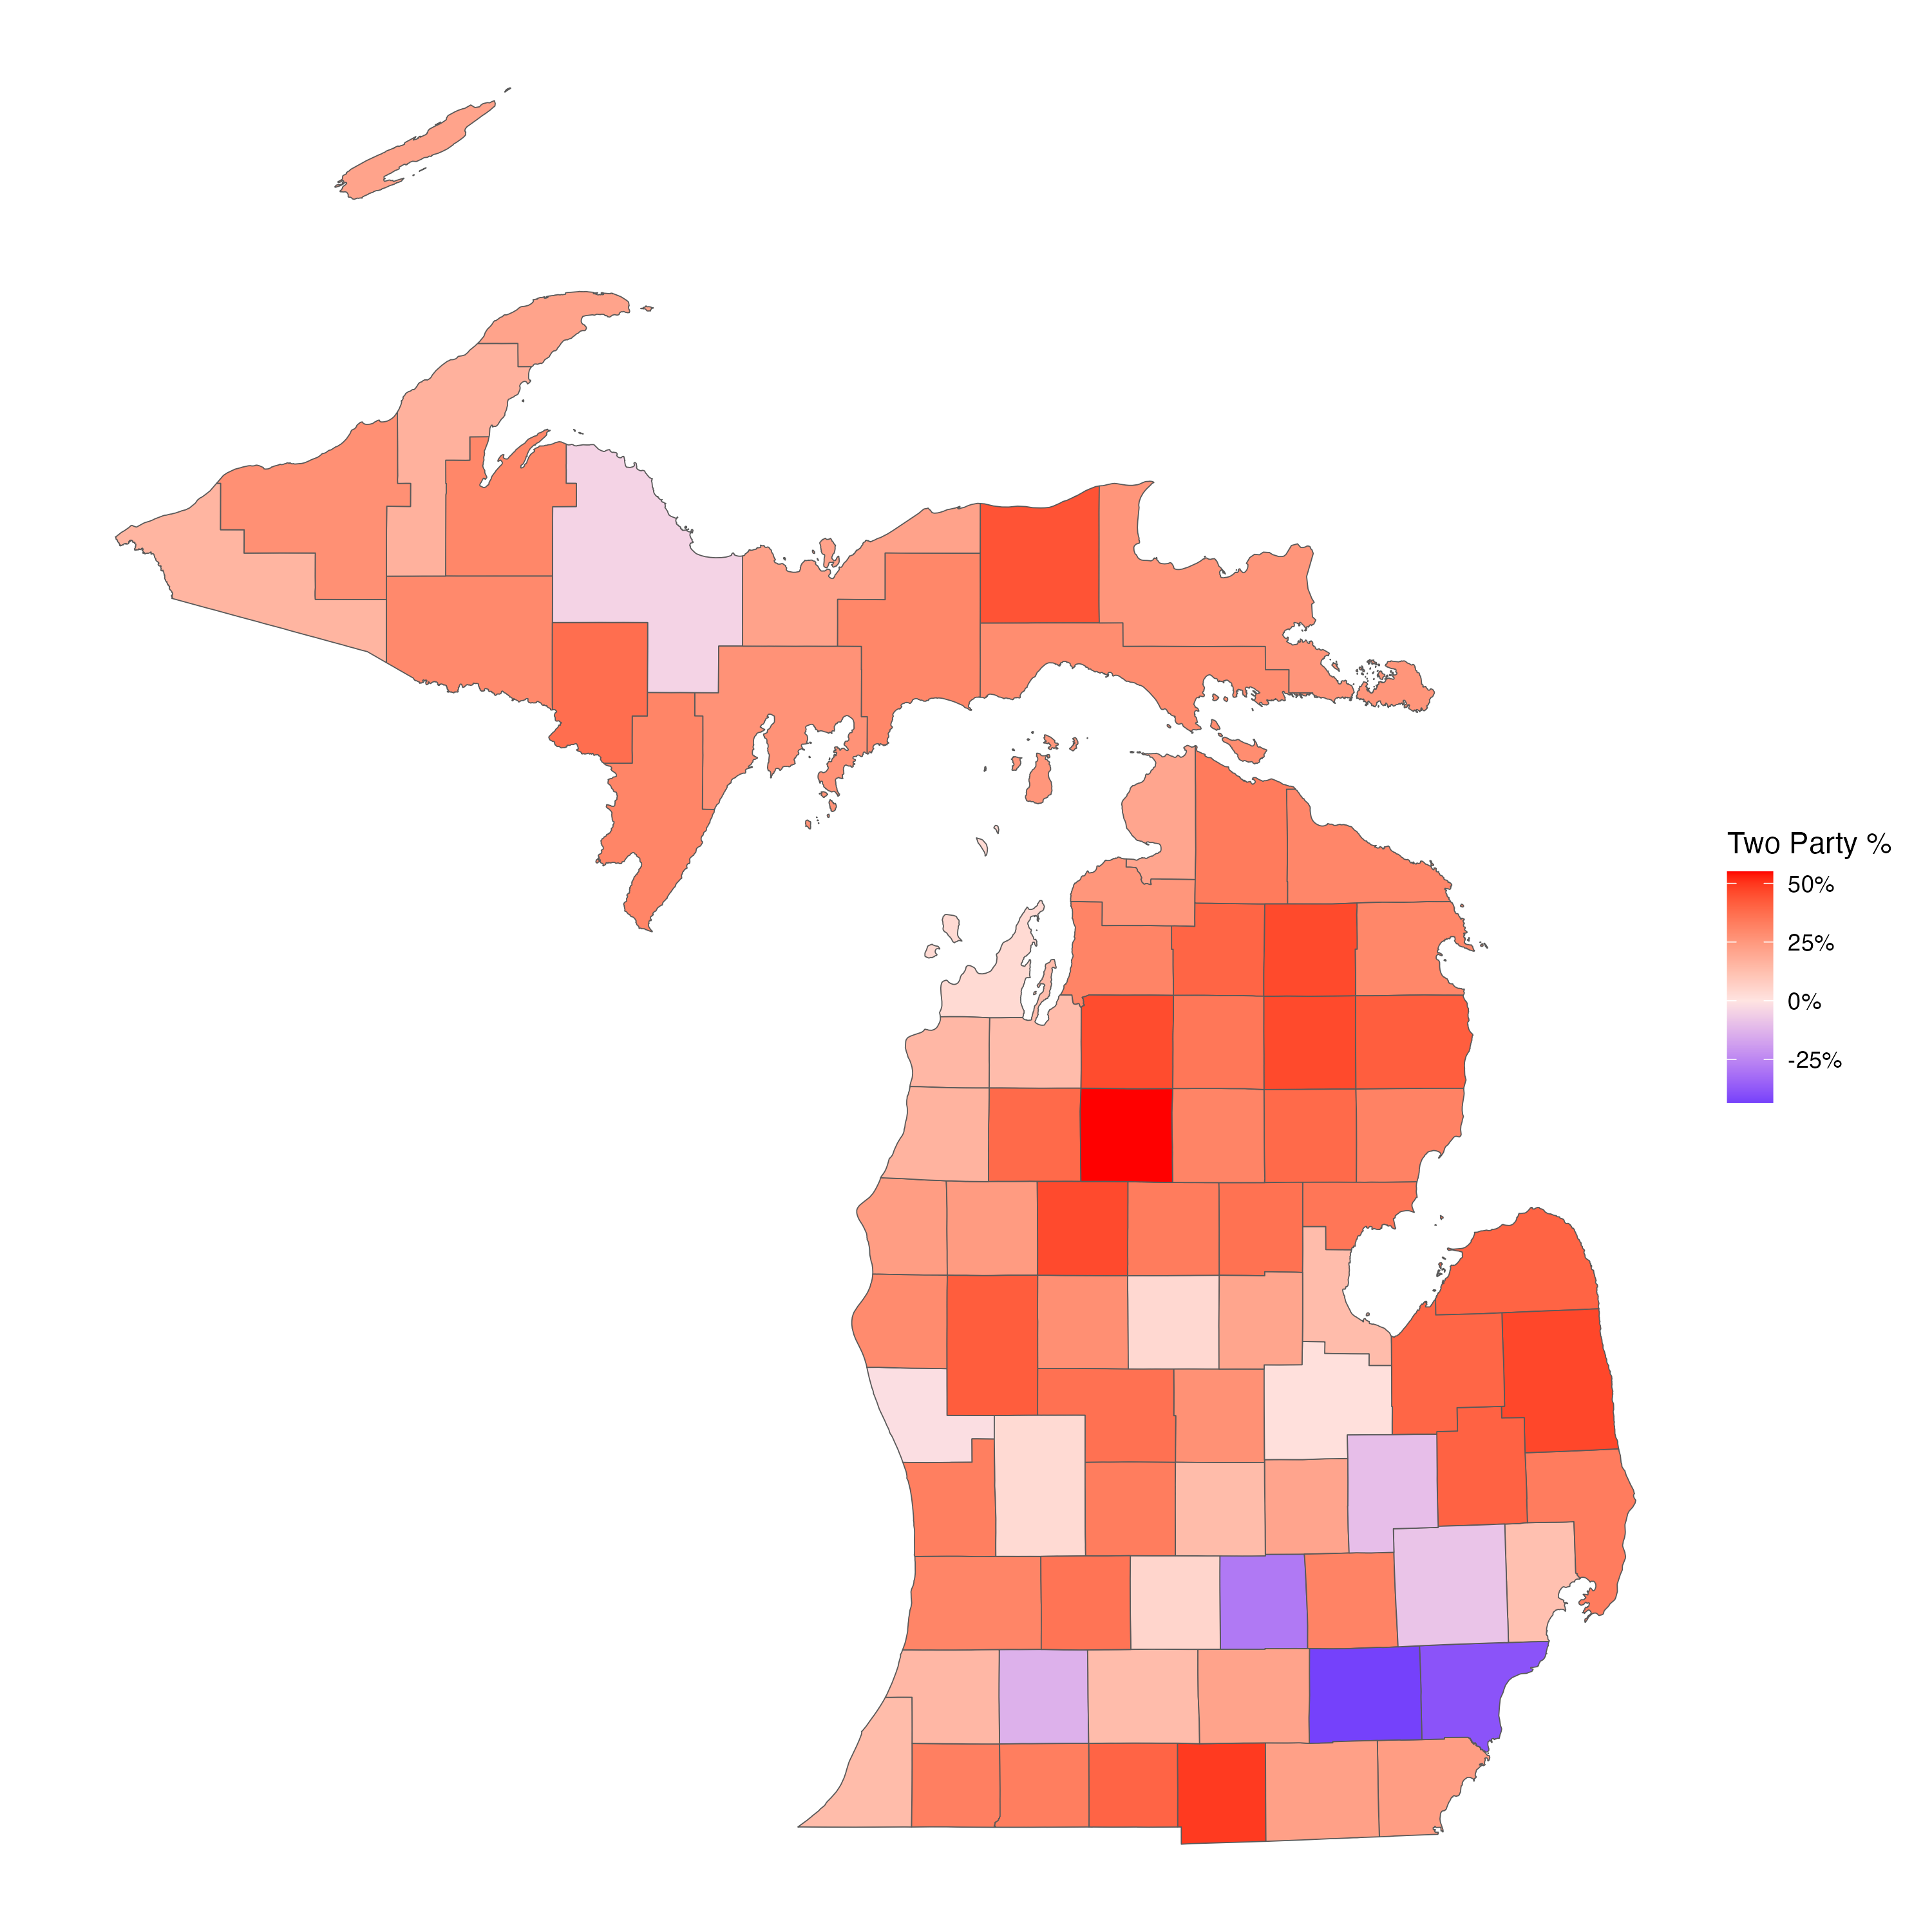
\includegraphics[width=0.9\textwidth]{plots/county-results.png}
    \caption{Michigan: 2016 Presidential Election Results by County}
    \label{fig:2016-results}
\end{figure}
\begin{figure}
    \centering
    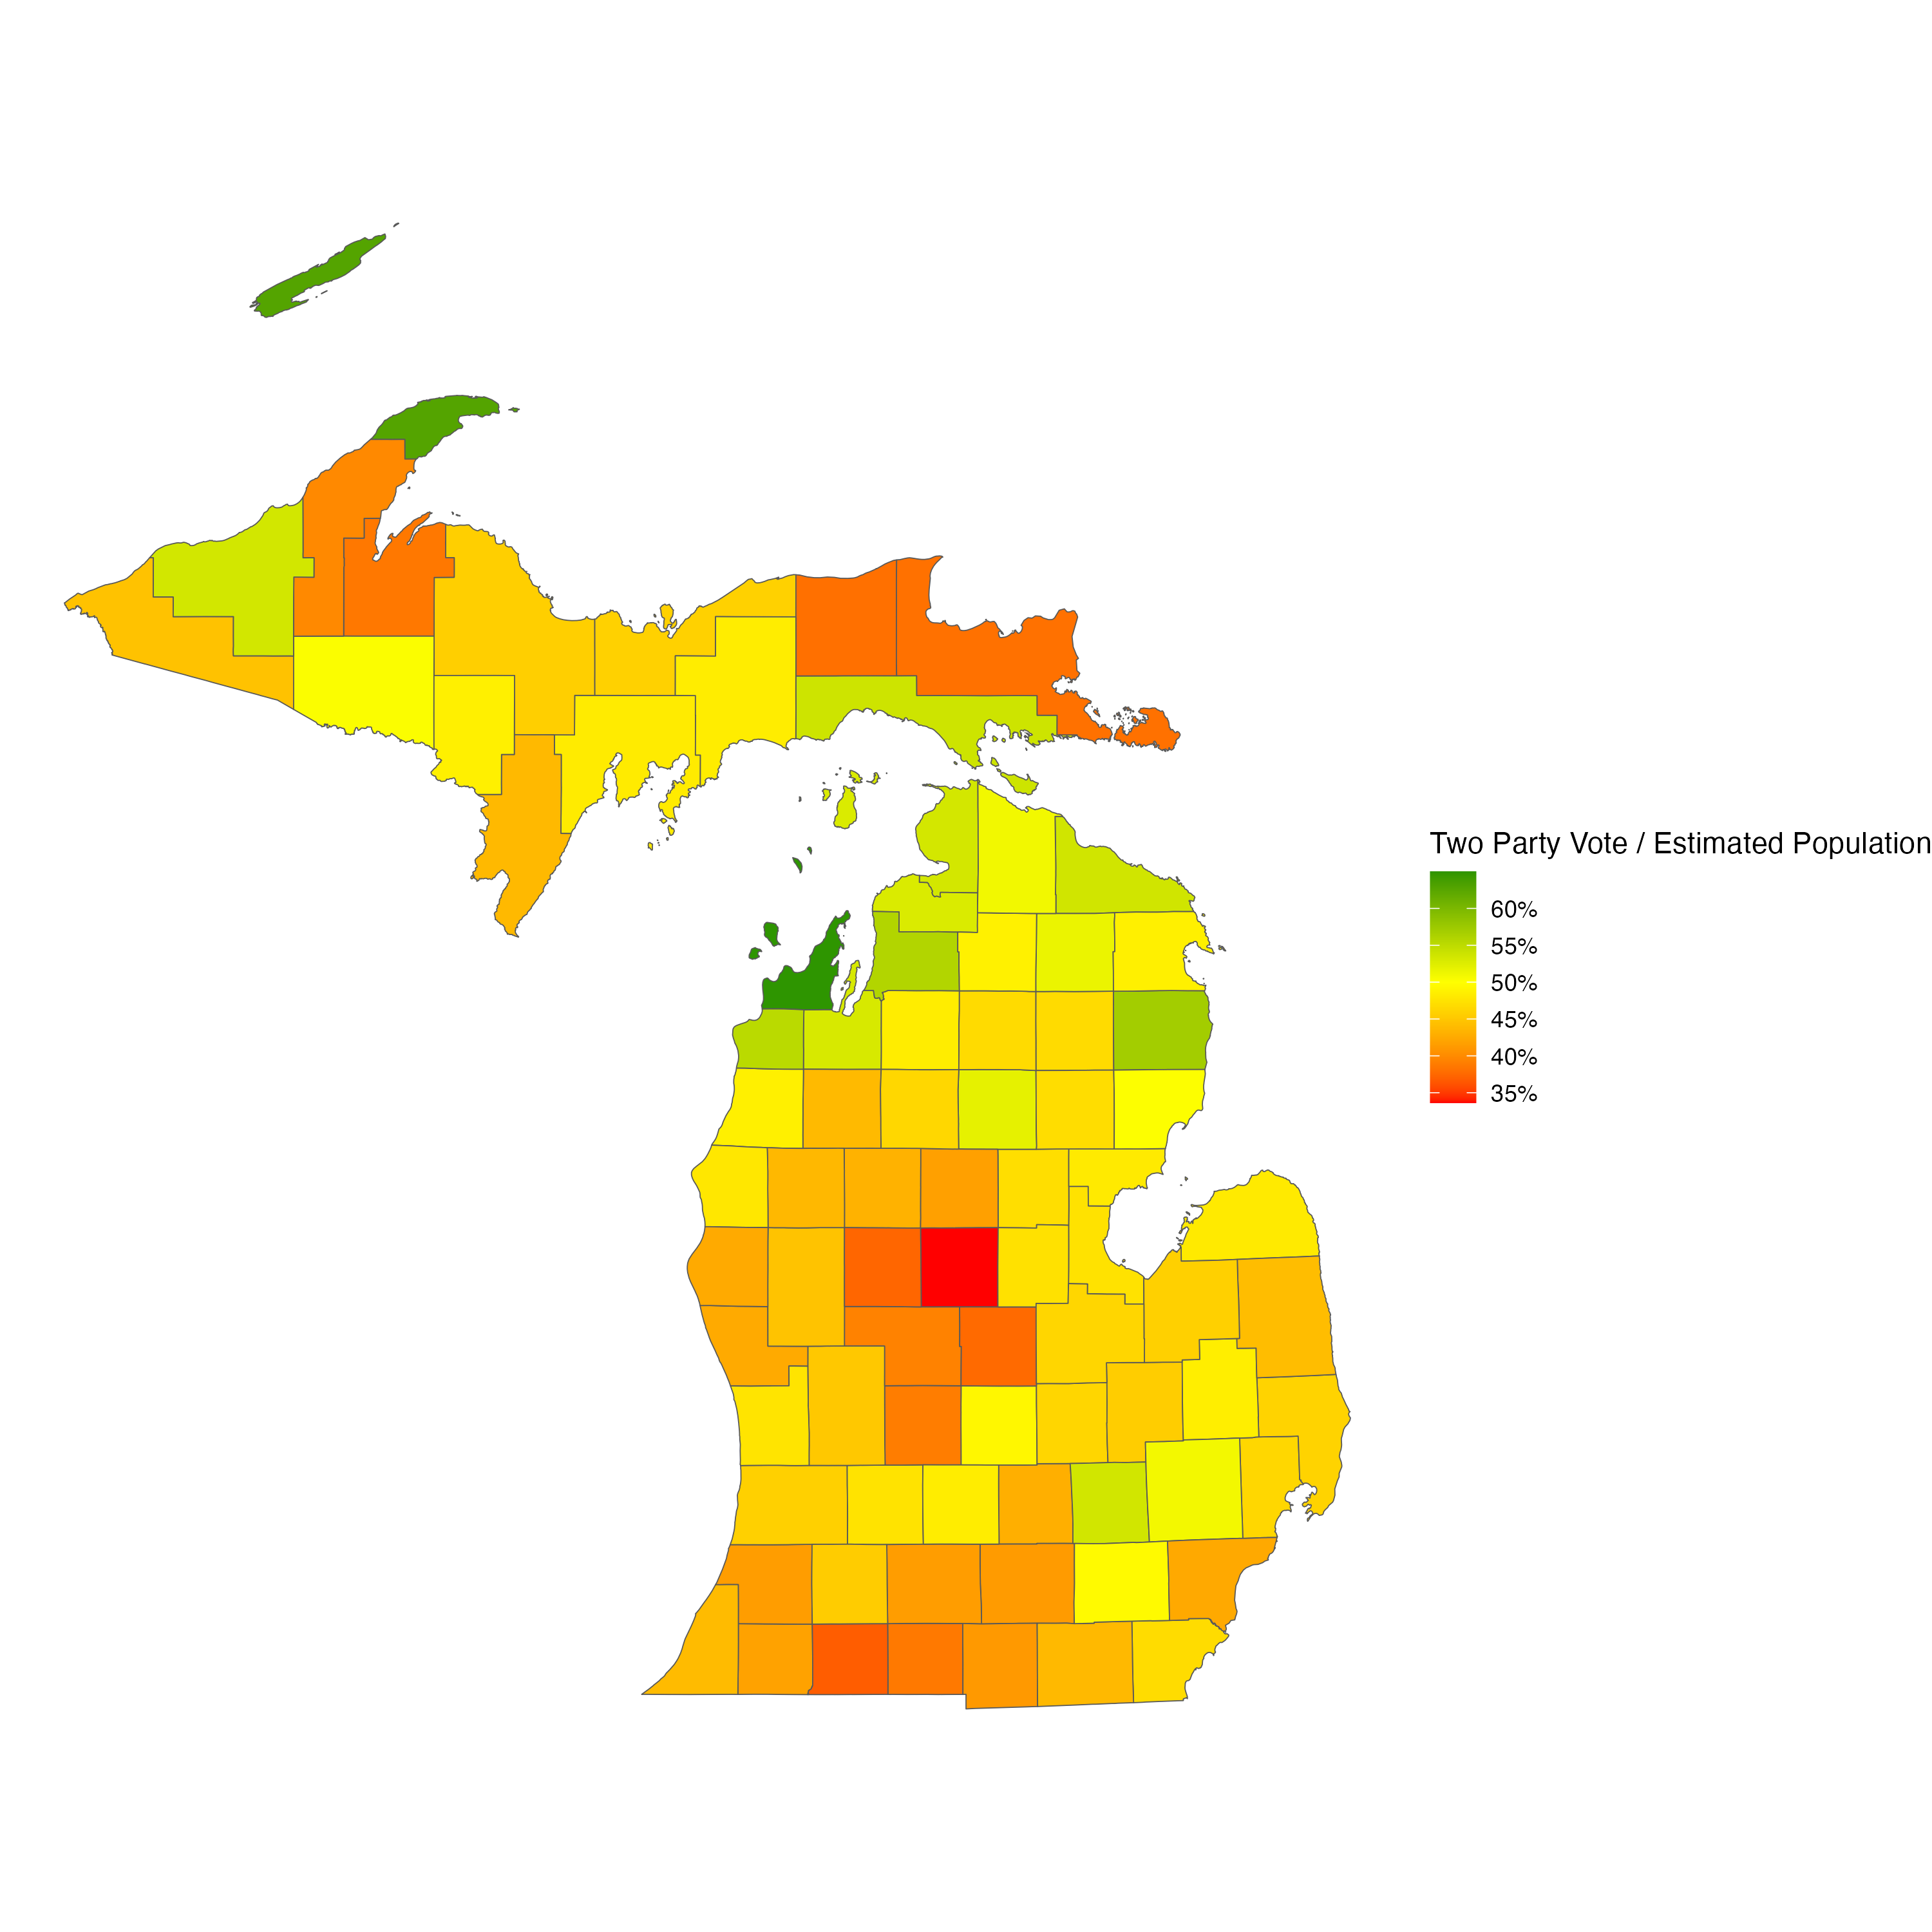
\includegraphics[width=0.9\textwidth]{plots/turnout.png}
    \caption{Michigan: Each County's Two Party Vote as a Percentage of its estimated population in the 2013-2017 American Community Survey}
    \label{fig:turnout}
\end{figure}
\begin{figure}
    \centering
    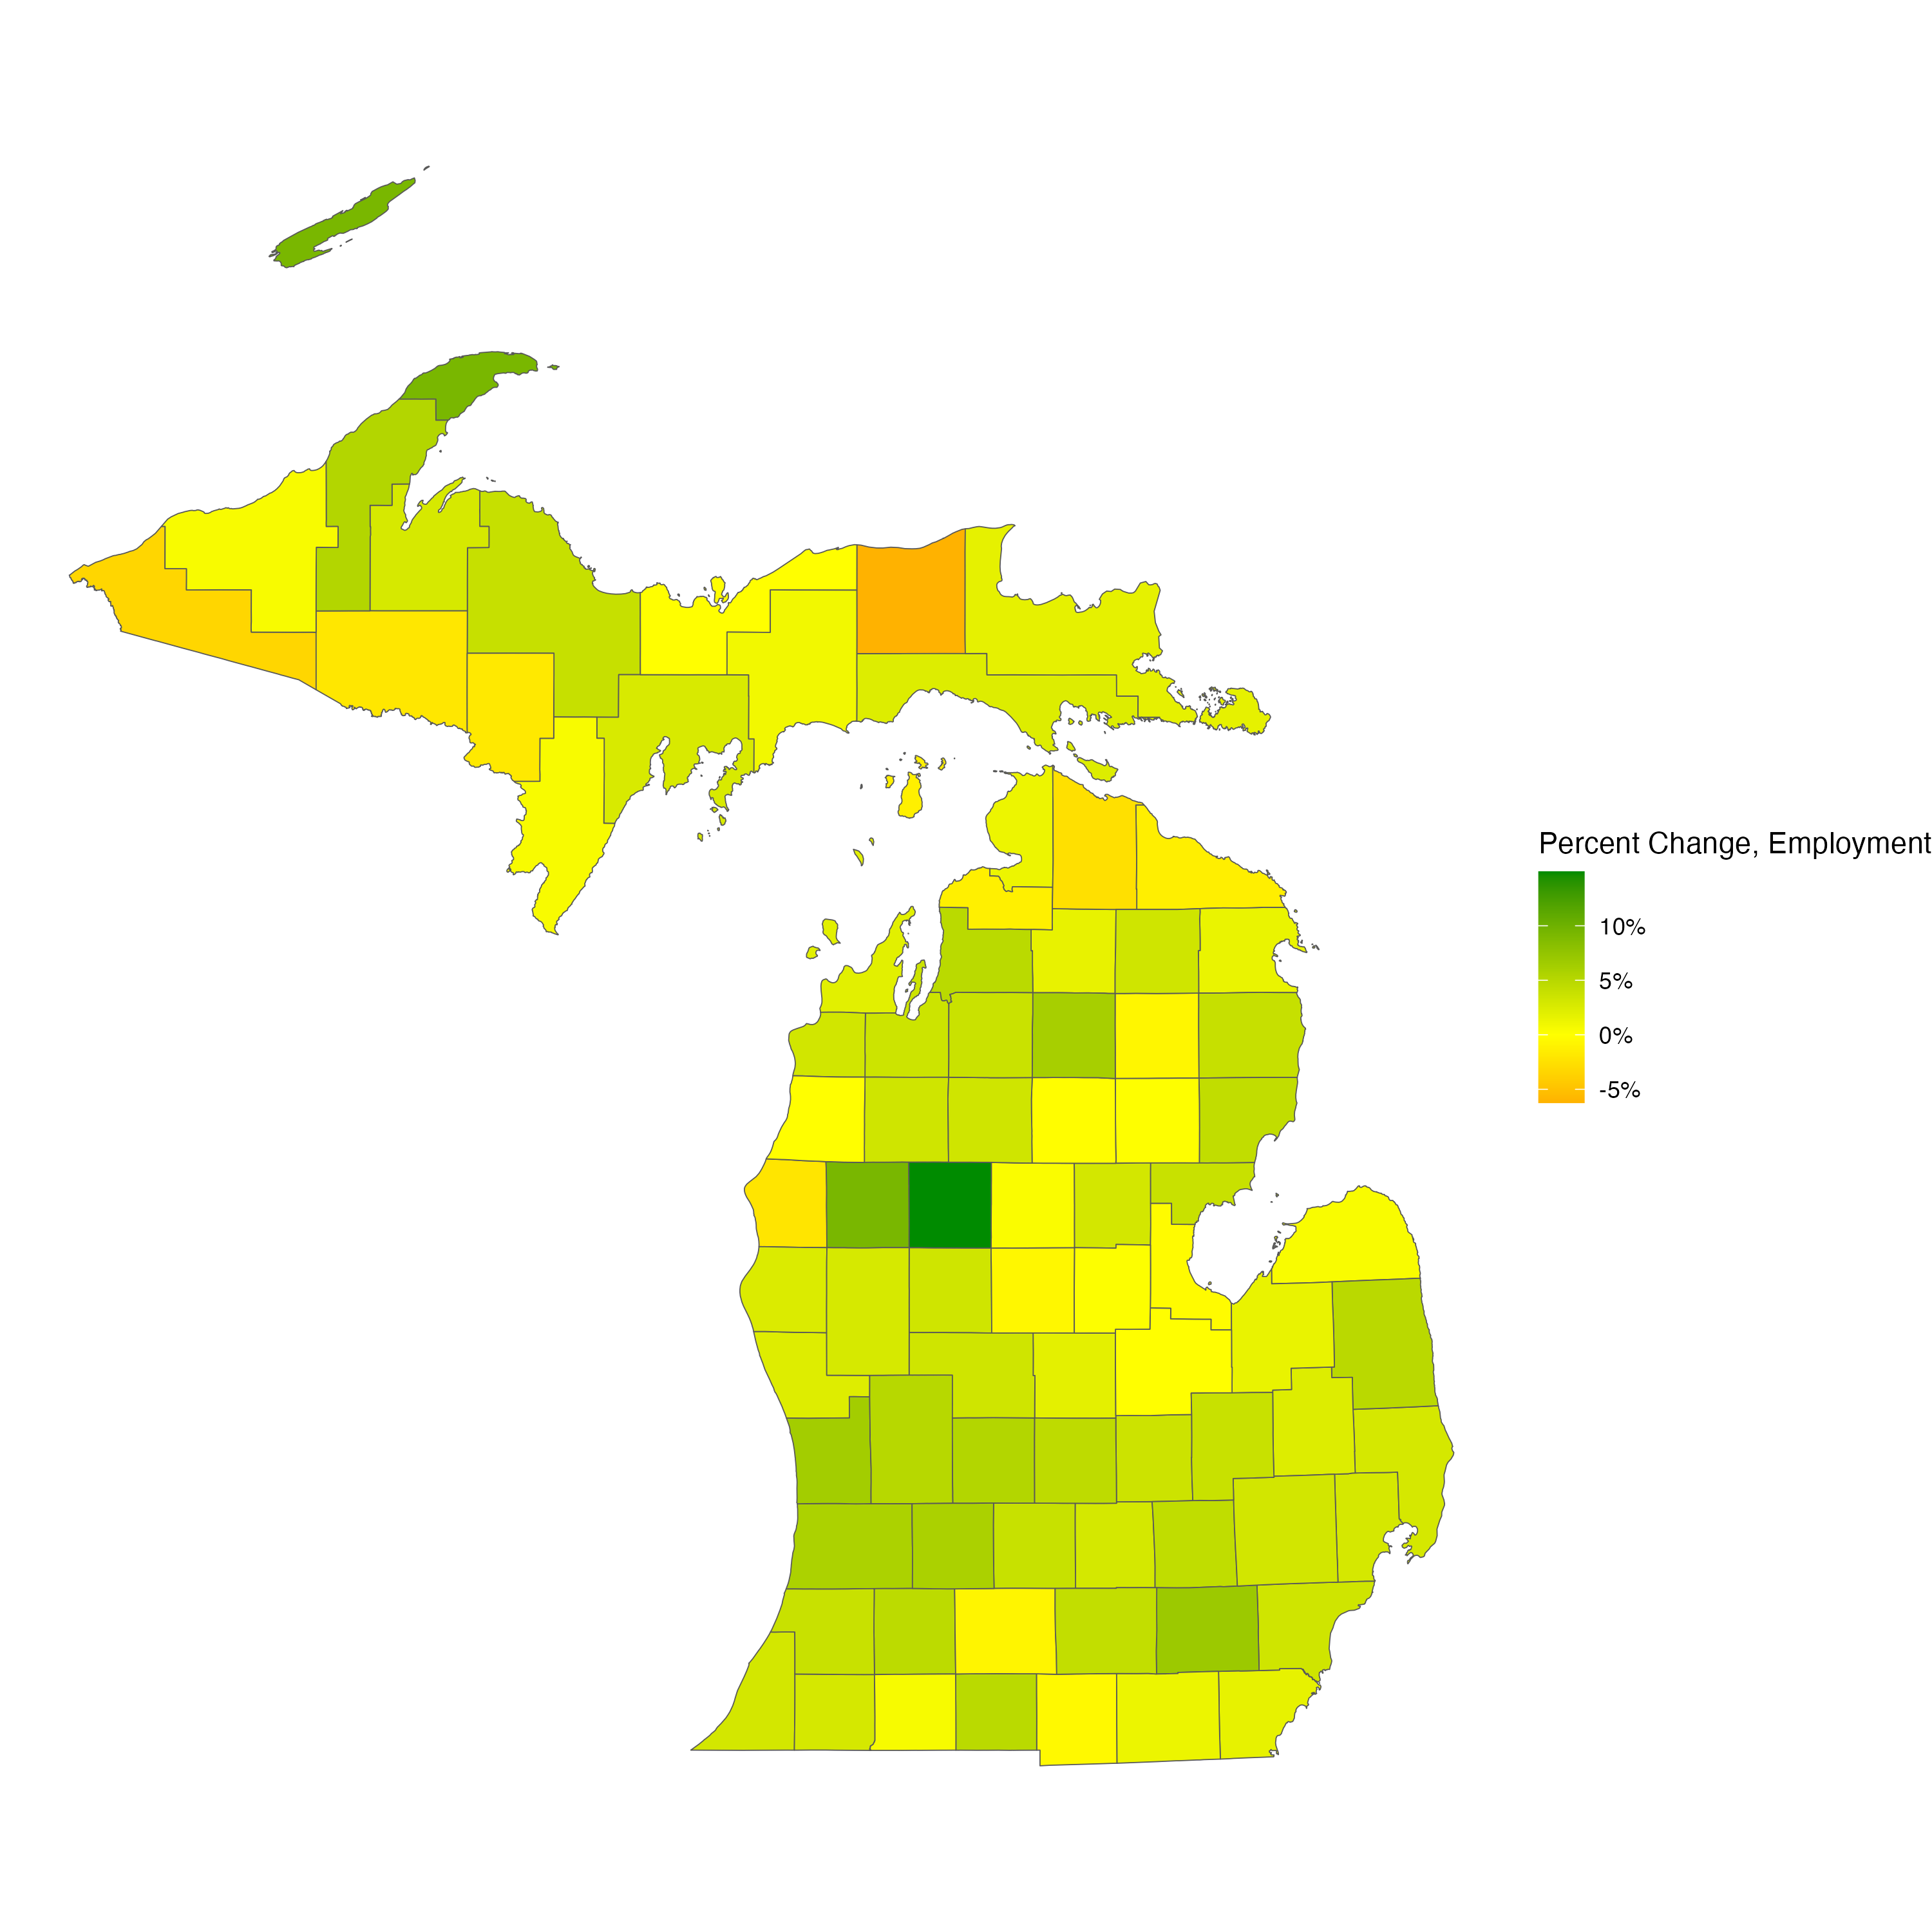
\includegraphics[width=0.9\textwidth]{plots/raw-employment-plot.png}
    \caption{Michigan: The percent change in the number of employed workers in each County from Trump's inauguration to February 2020, the Month before the pandemic hit}
\end{figure}
\begin{figure}
    \centering
    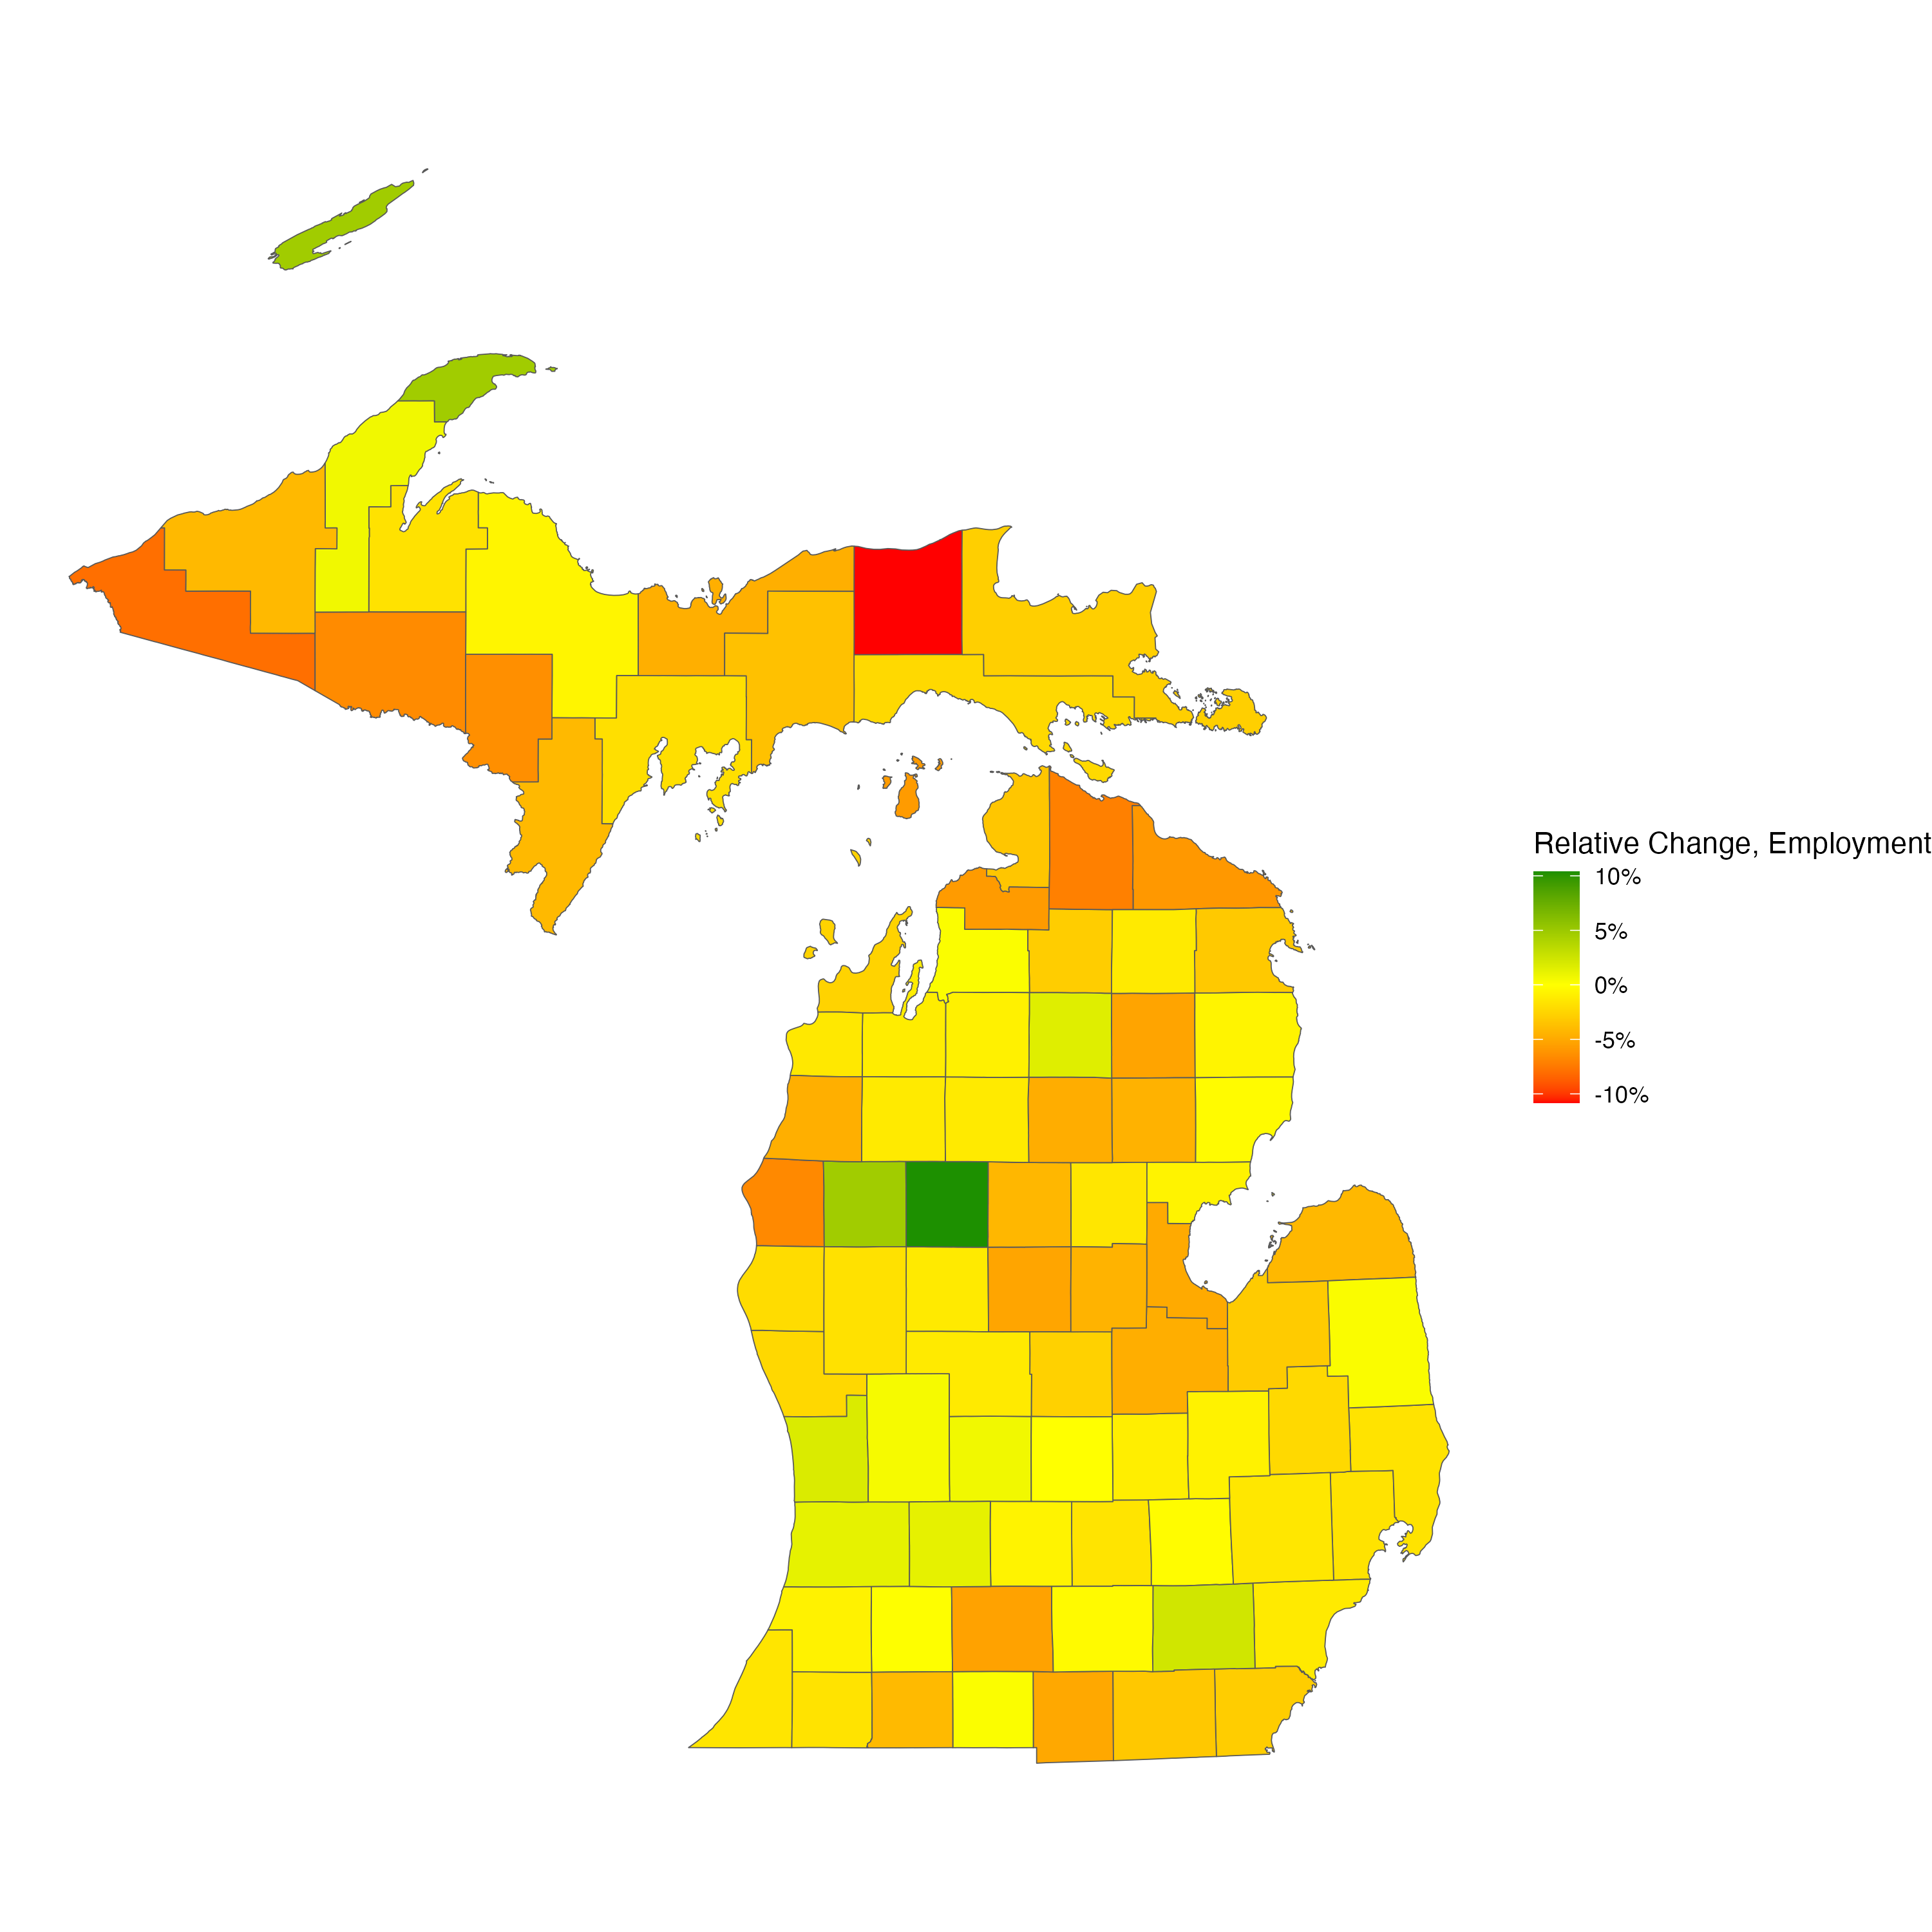
\includegraphics[width=0.9\textwidth]{plots/relative-employment-plot.png}
    \caption{Michigan: The percent change in the number of employed workers in each county in Michigan minus the national percent change in the number of employed workers over the period from Trump's inauguration to February 2020}
\end{figure}
\begin{figure}
    \centering
    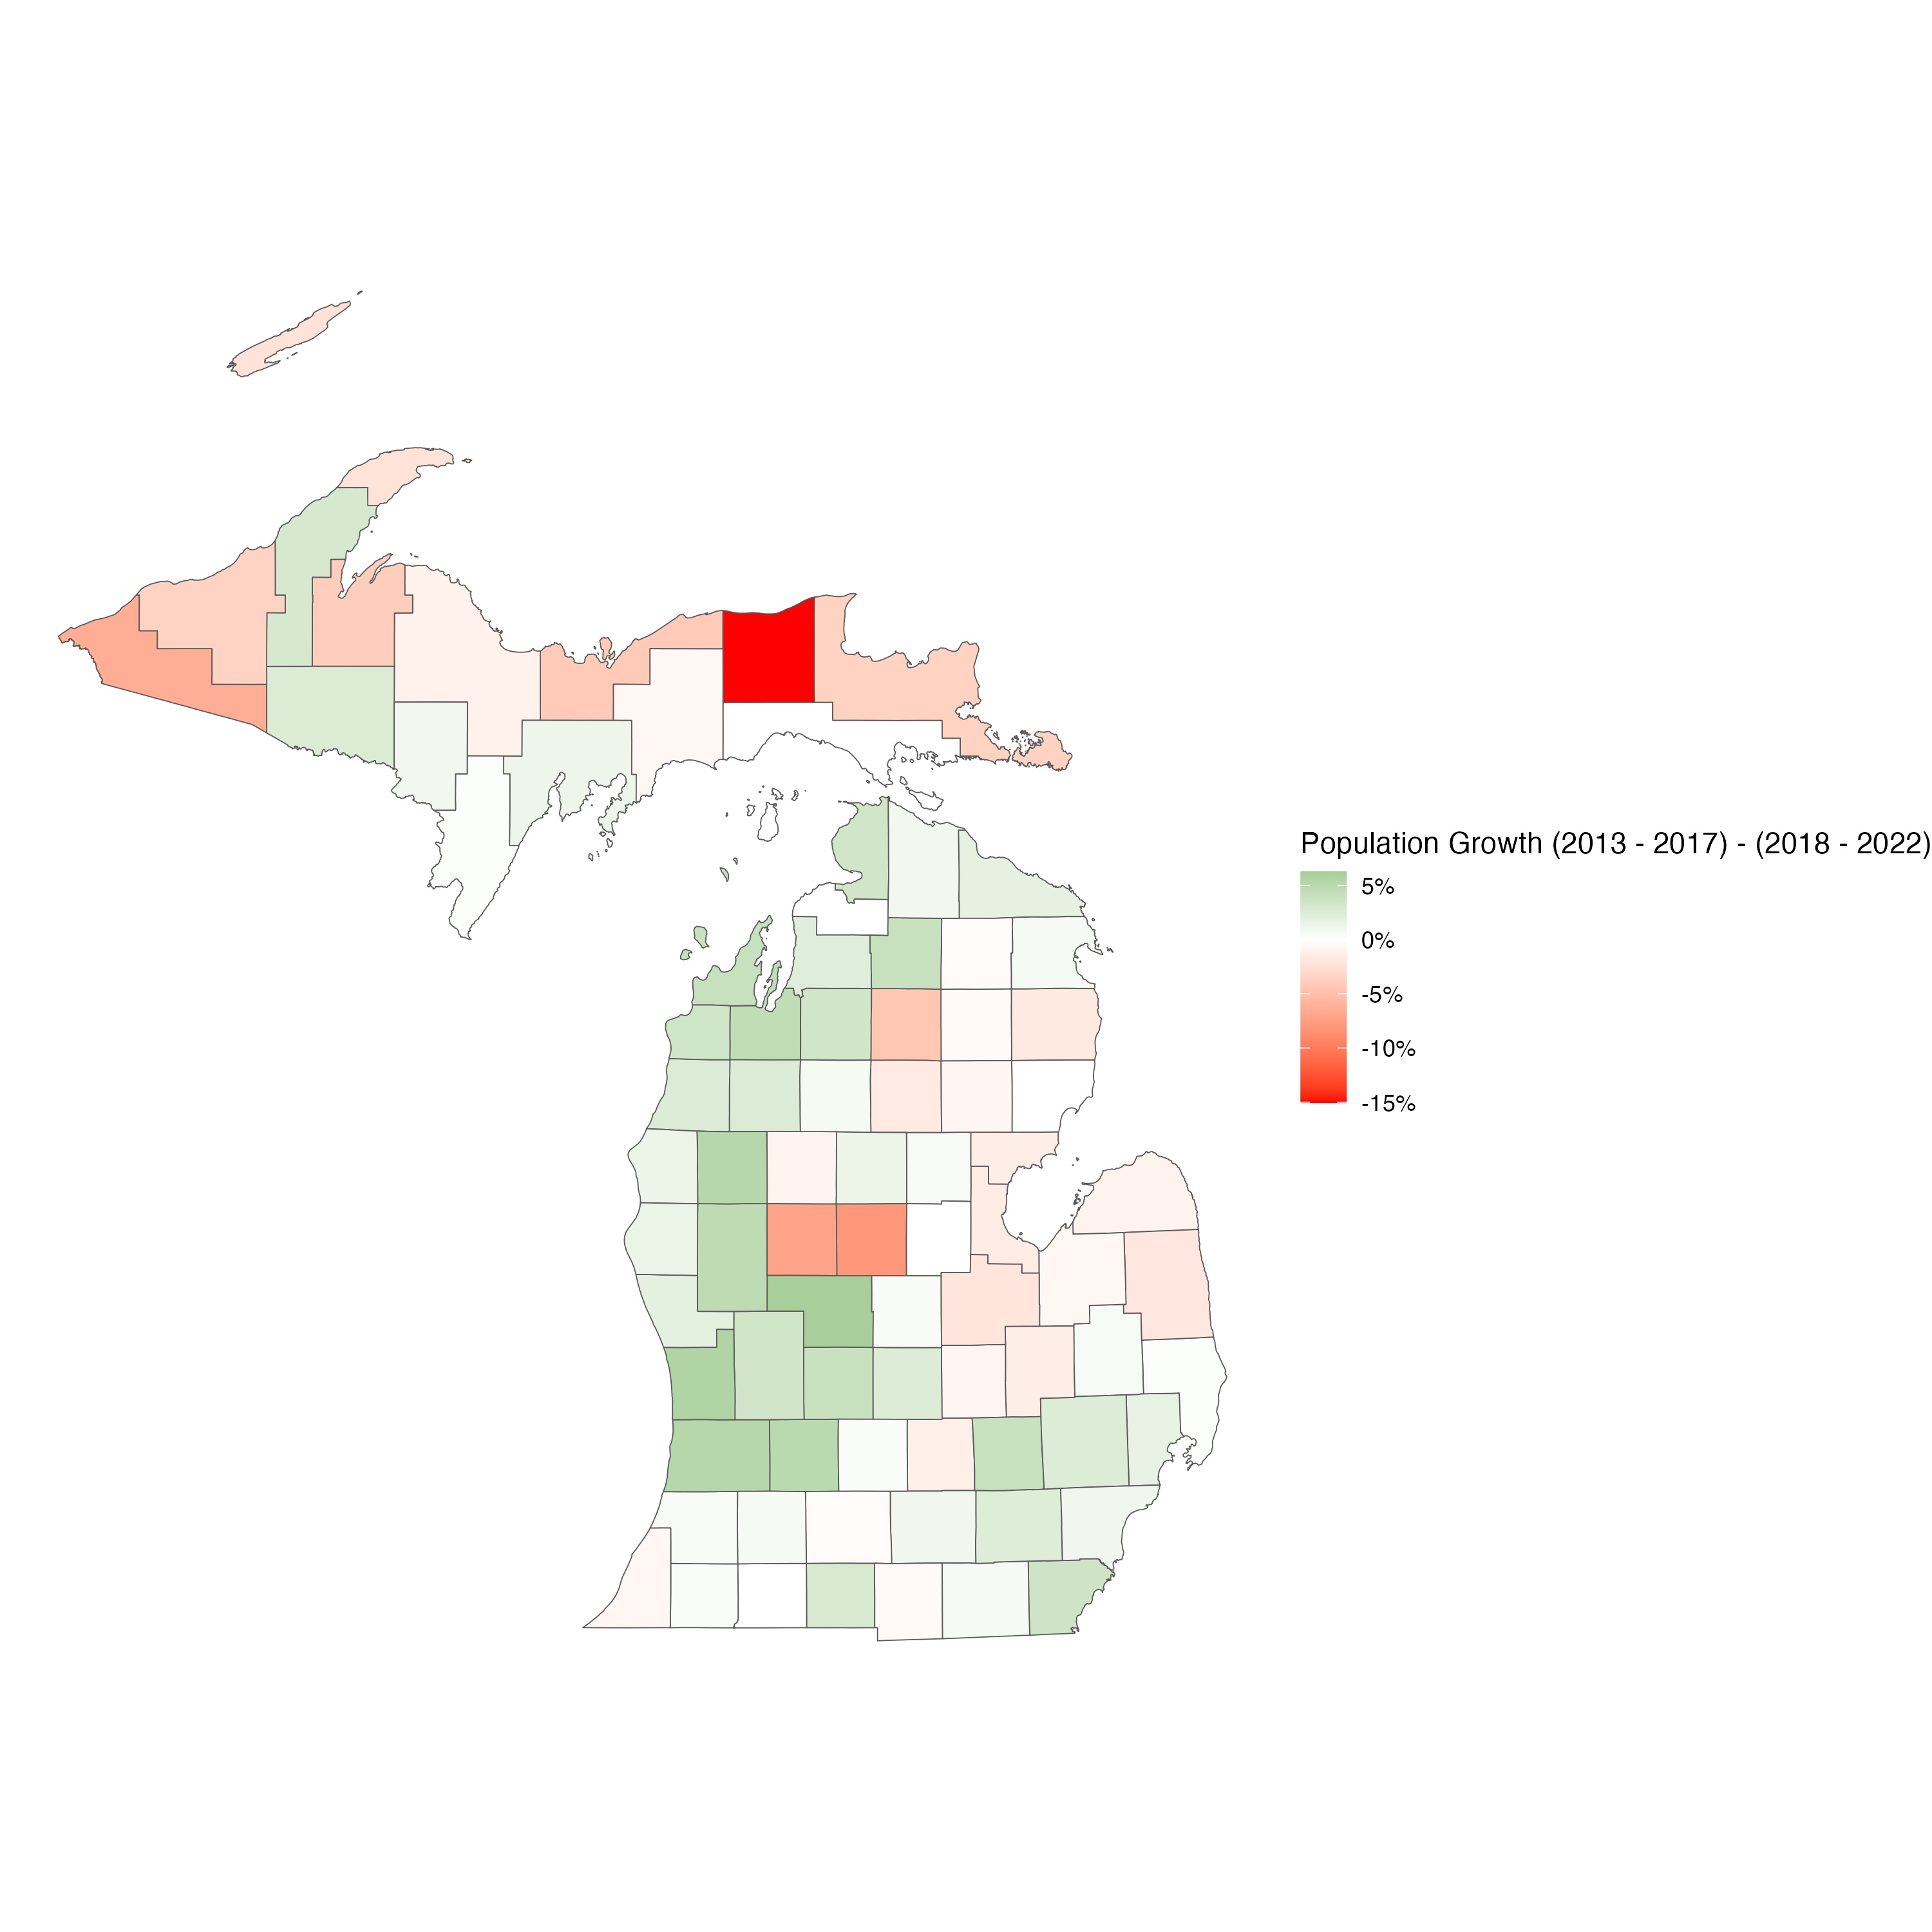
\includegraphics[width=0.9\textwidth]{plots/mi-growth.png}
    \caption{Michigan: County level population growth from the 2017 ACS to the 2022 ACS}
\end{figure}
\begin{figure}
    \centering
    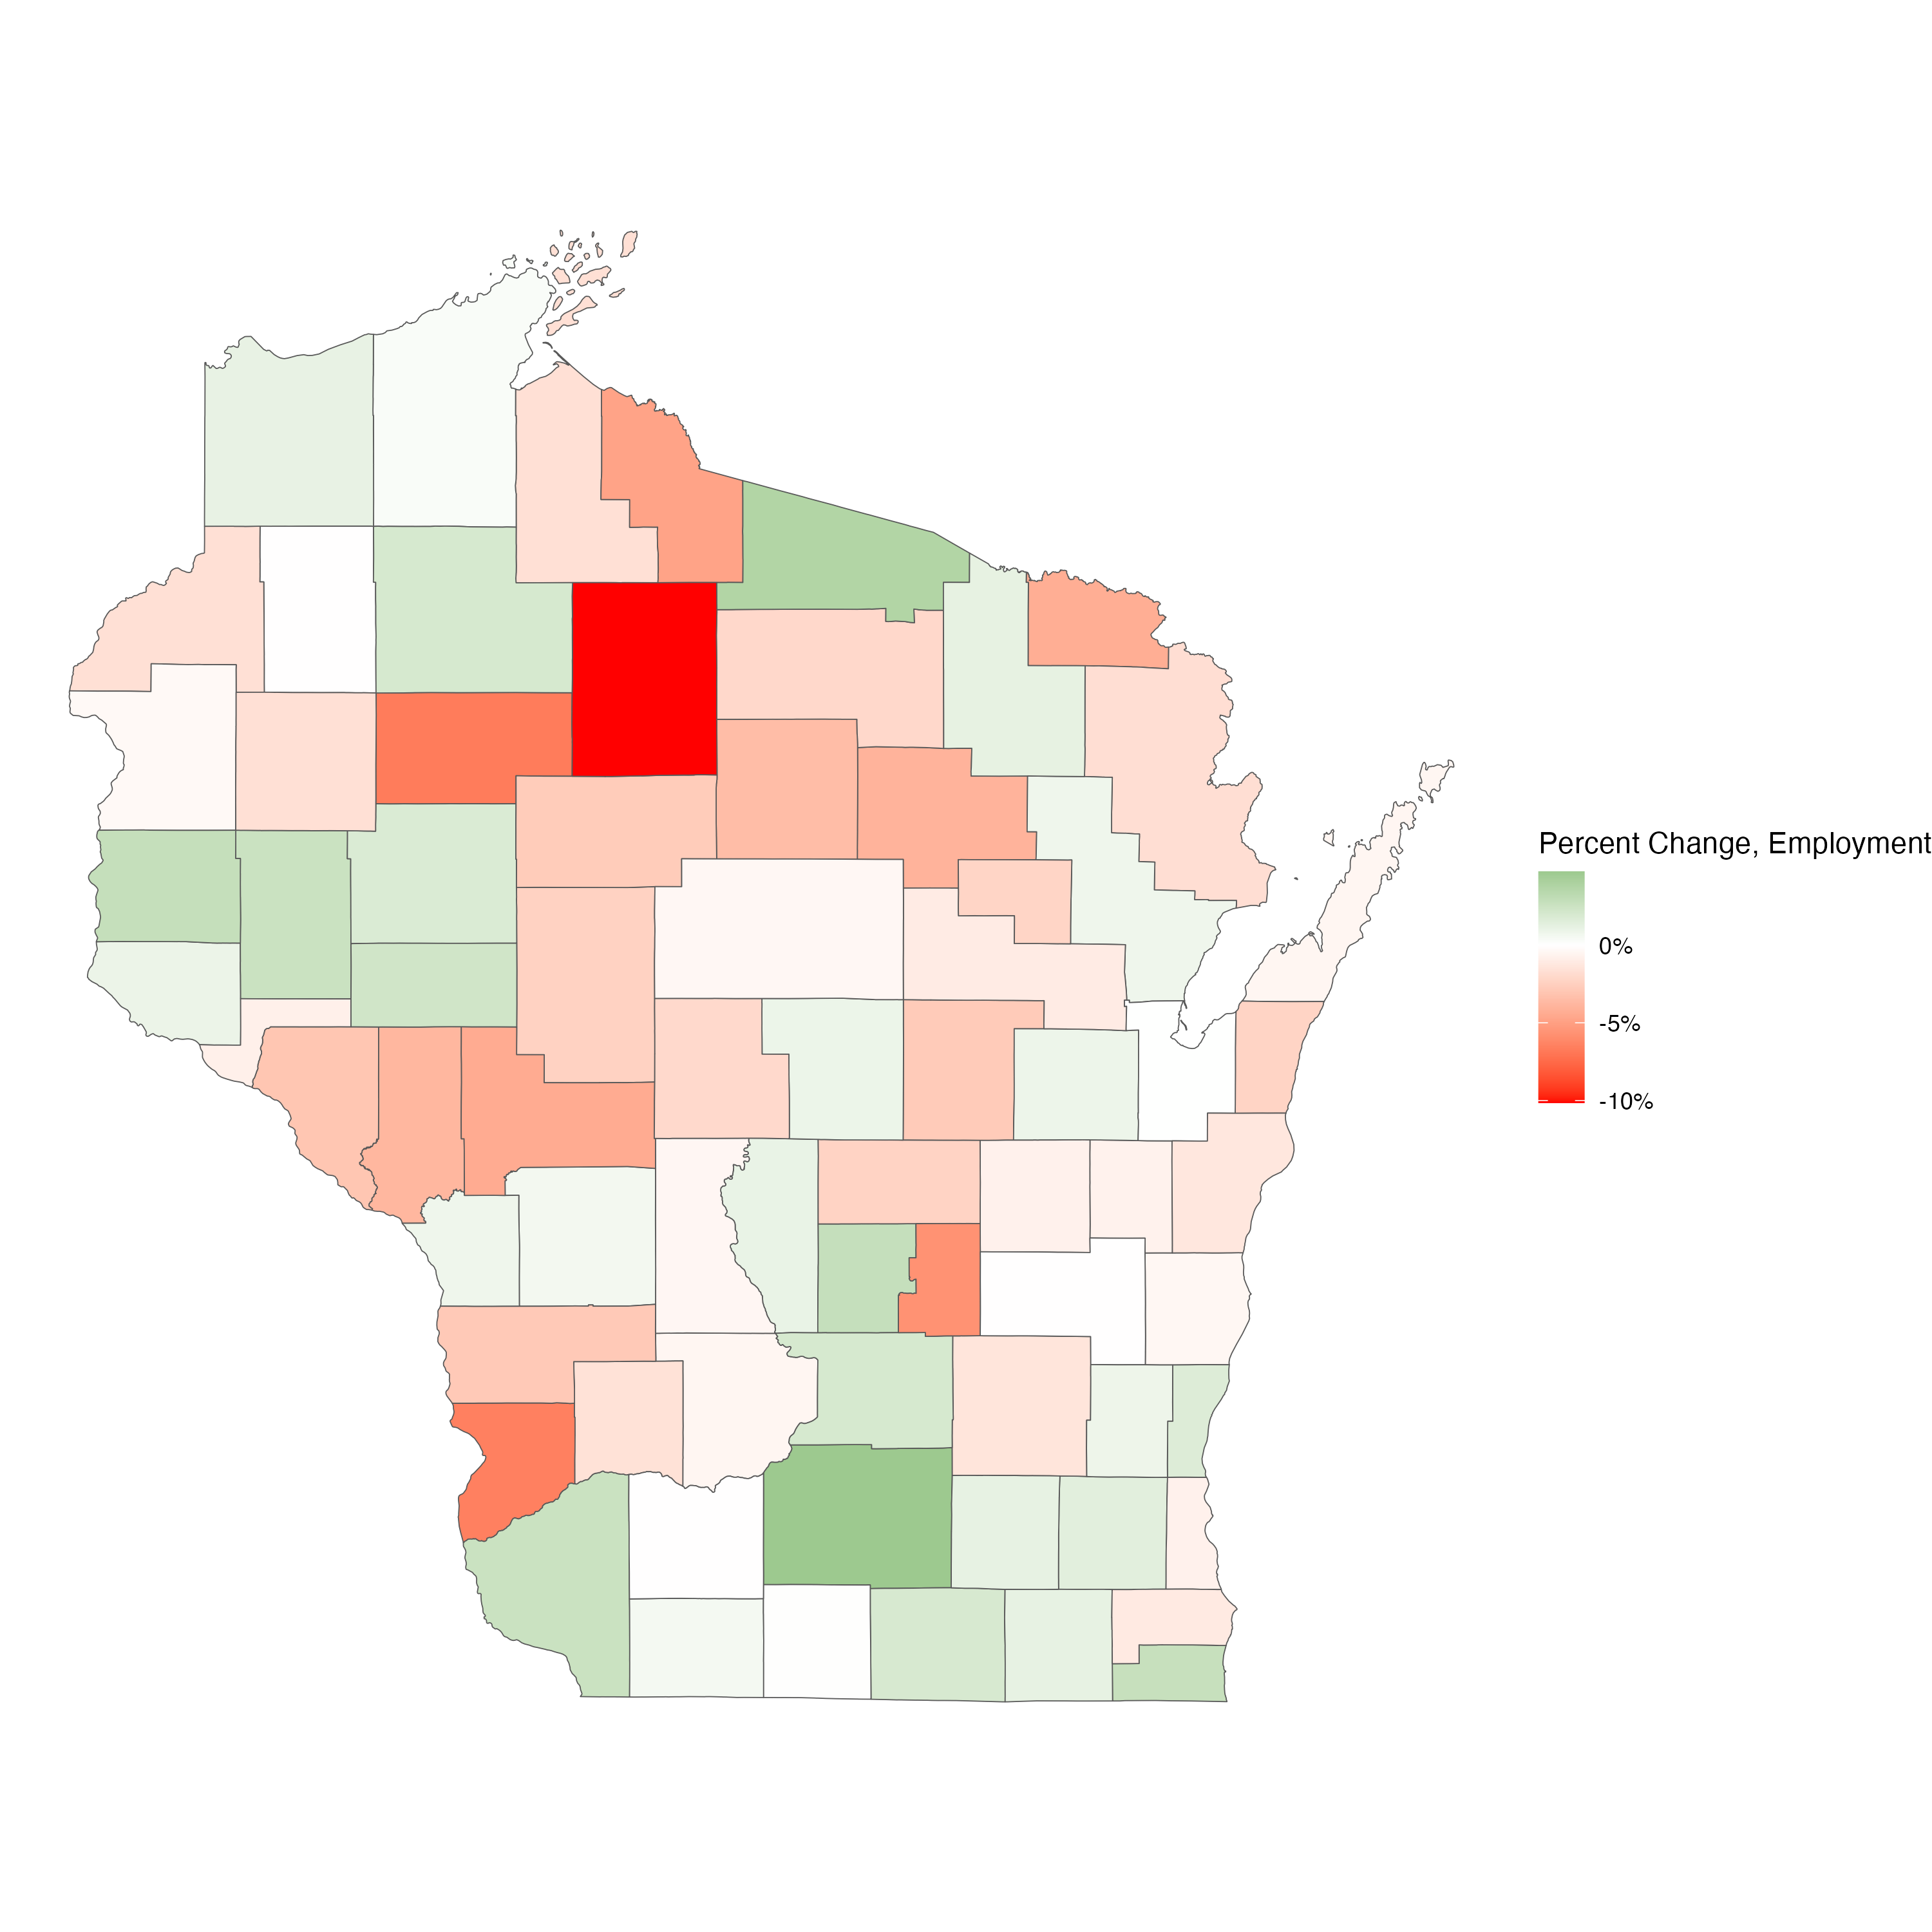
\includegraphics[width=0.9\textwidth]{plots/raw-employment-plot-wi.png}
    \caption{Wisconsin: The percent change in the number of employed workers in each County from Trump's inauguration to February 2020, the Month before the pandemic hit}
\end{figure}
\begin{figure}
    \centering
    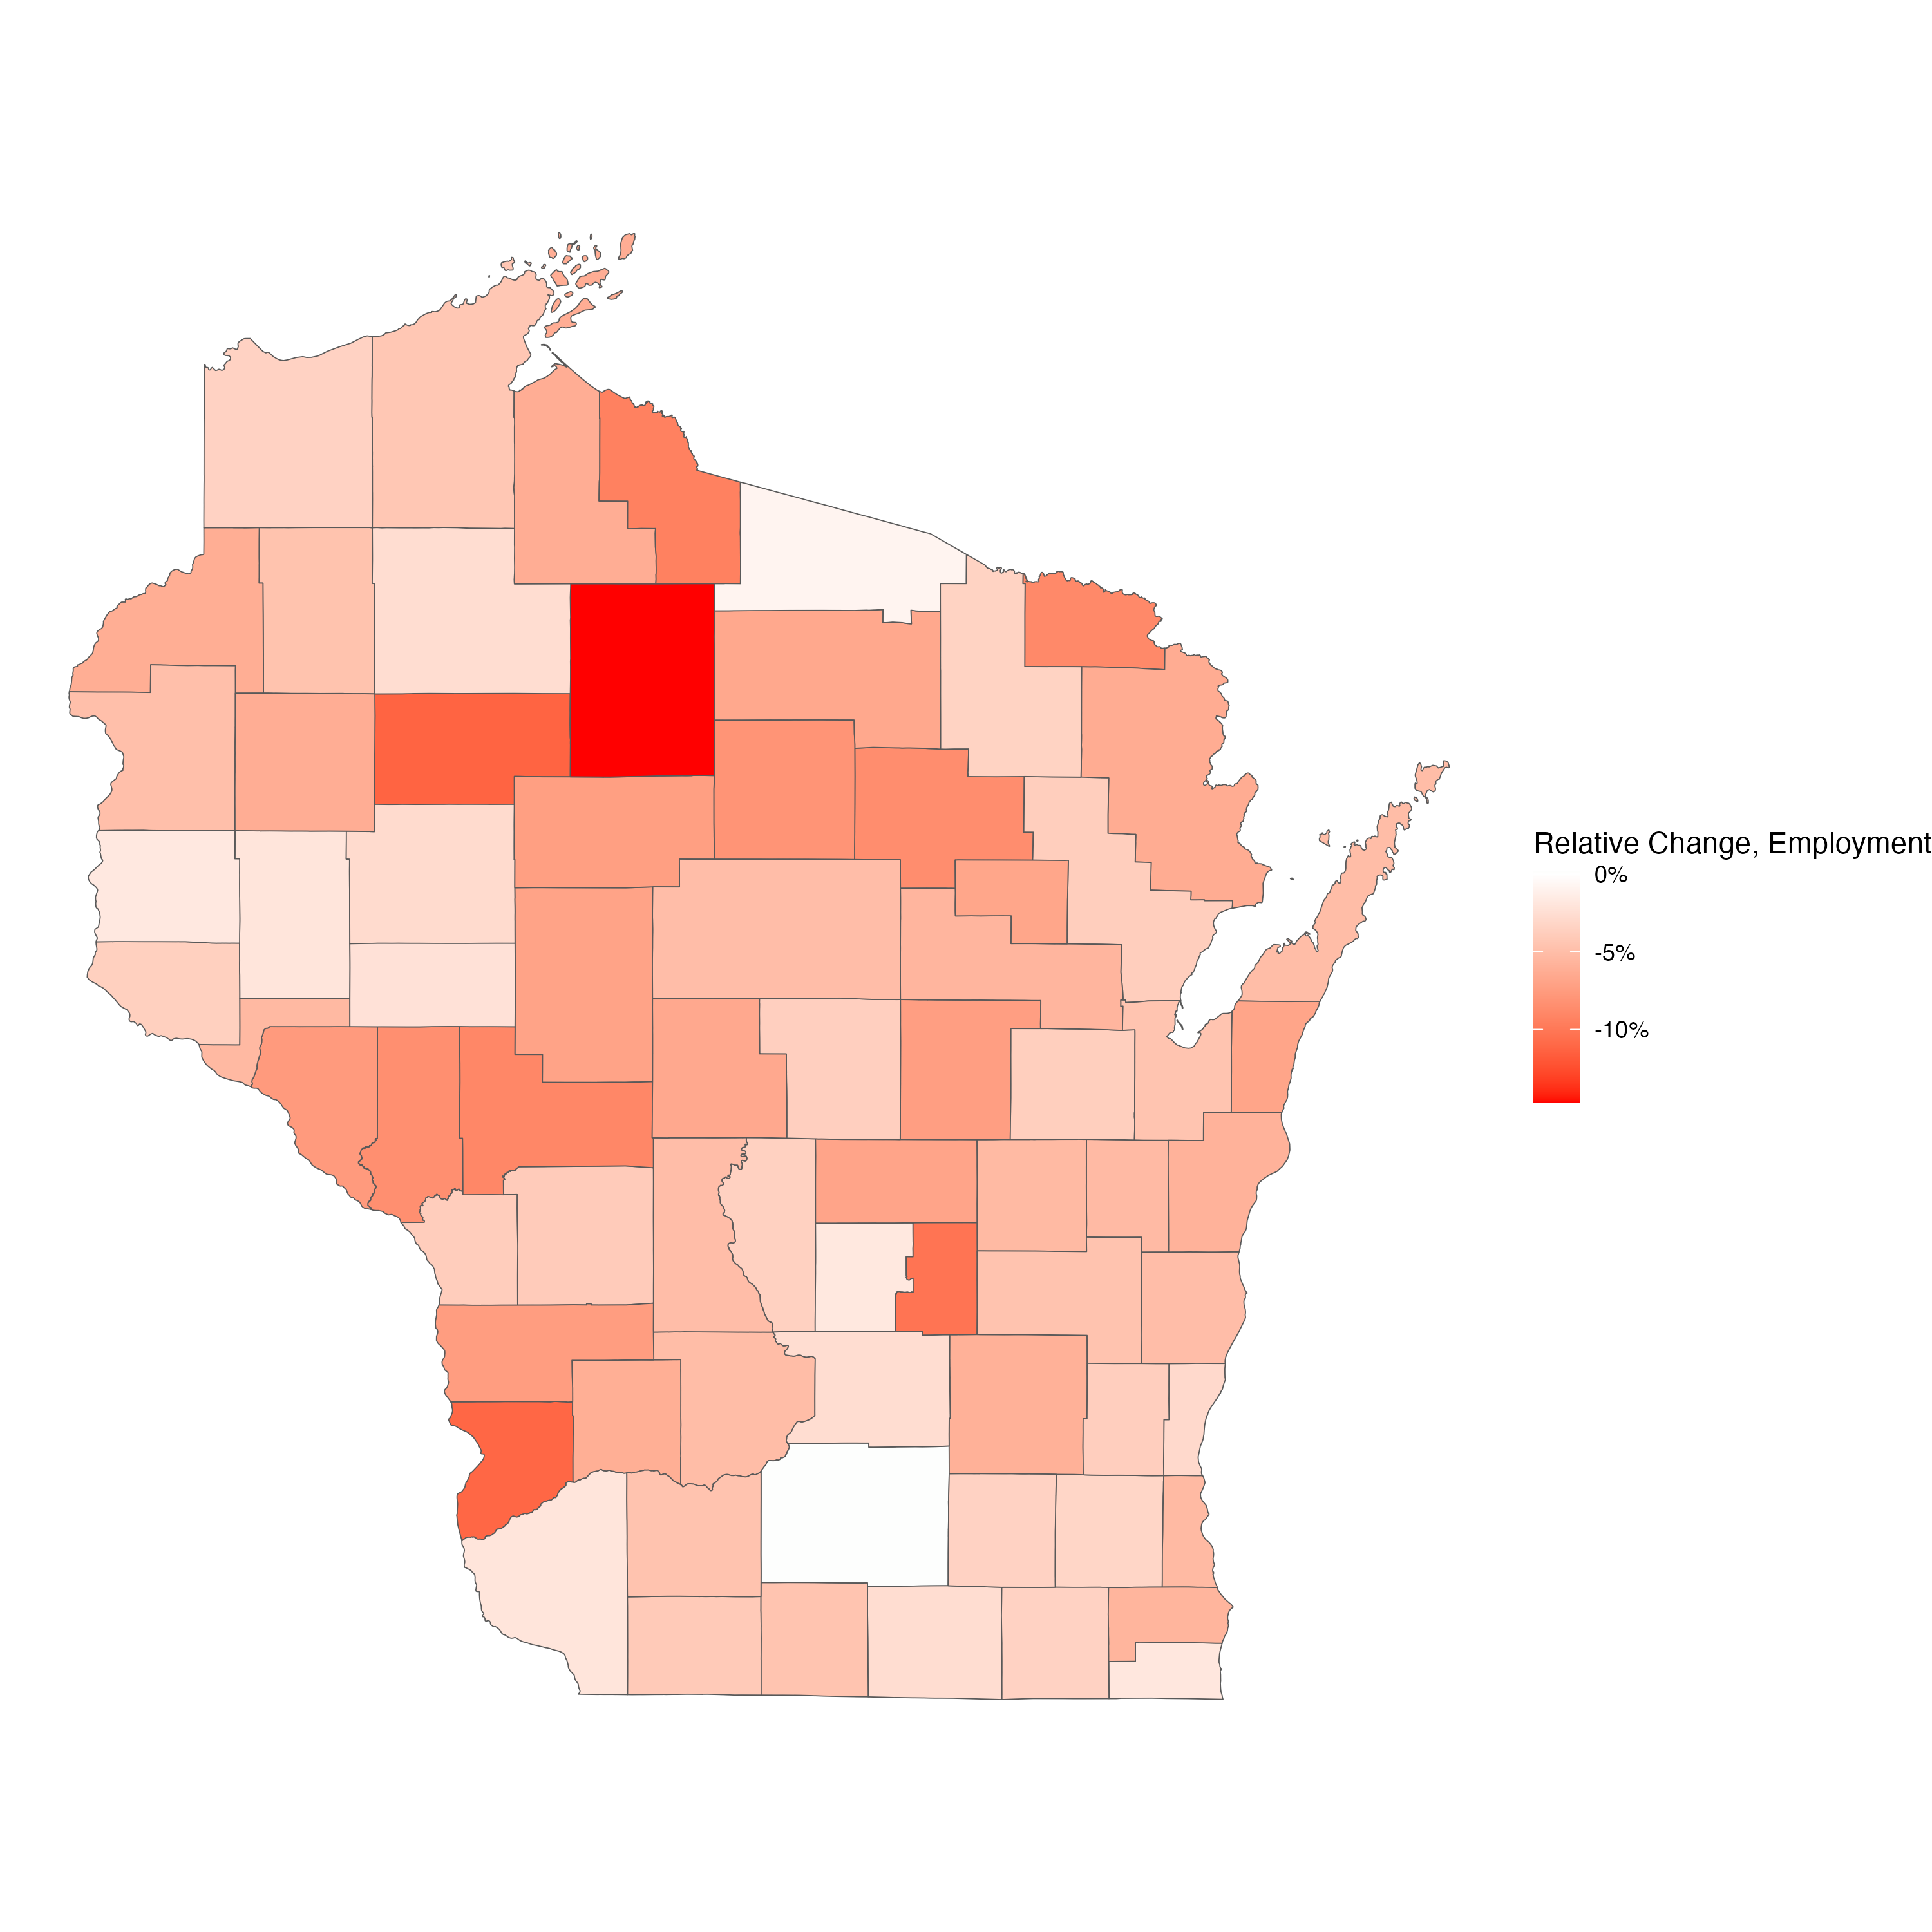
\includegraphics[width=0.9\textwidth]{plots/relative-employment-plot-wi.png}
    \caption{The percent change in the number of employed workers in each county in Wisconsin minus the national percent change in the number of employed workers over the period from Trump's inauguration to February 2020}
\end{figure}
\begin{figure}
    \centering
    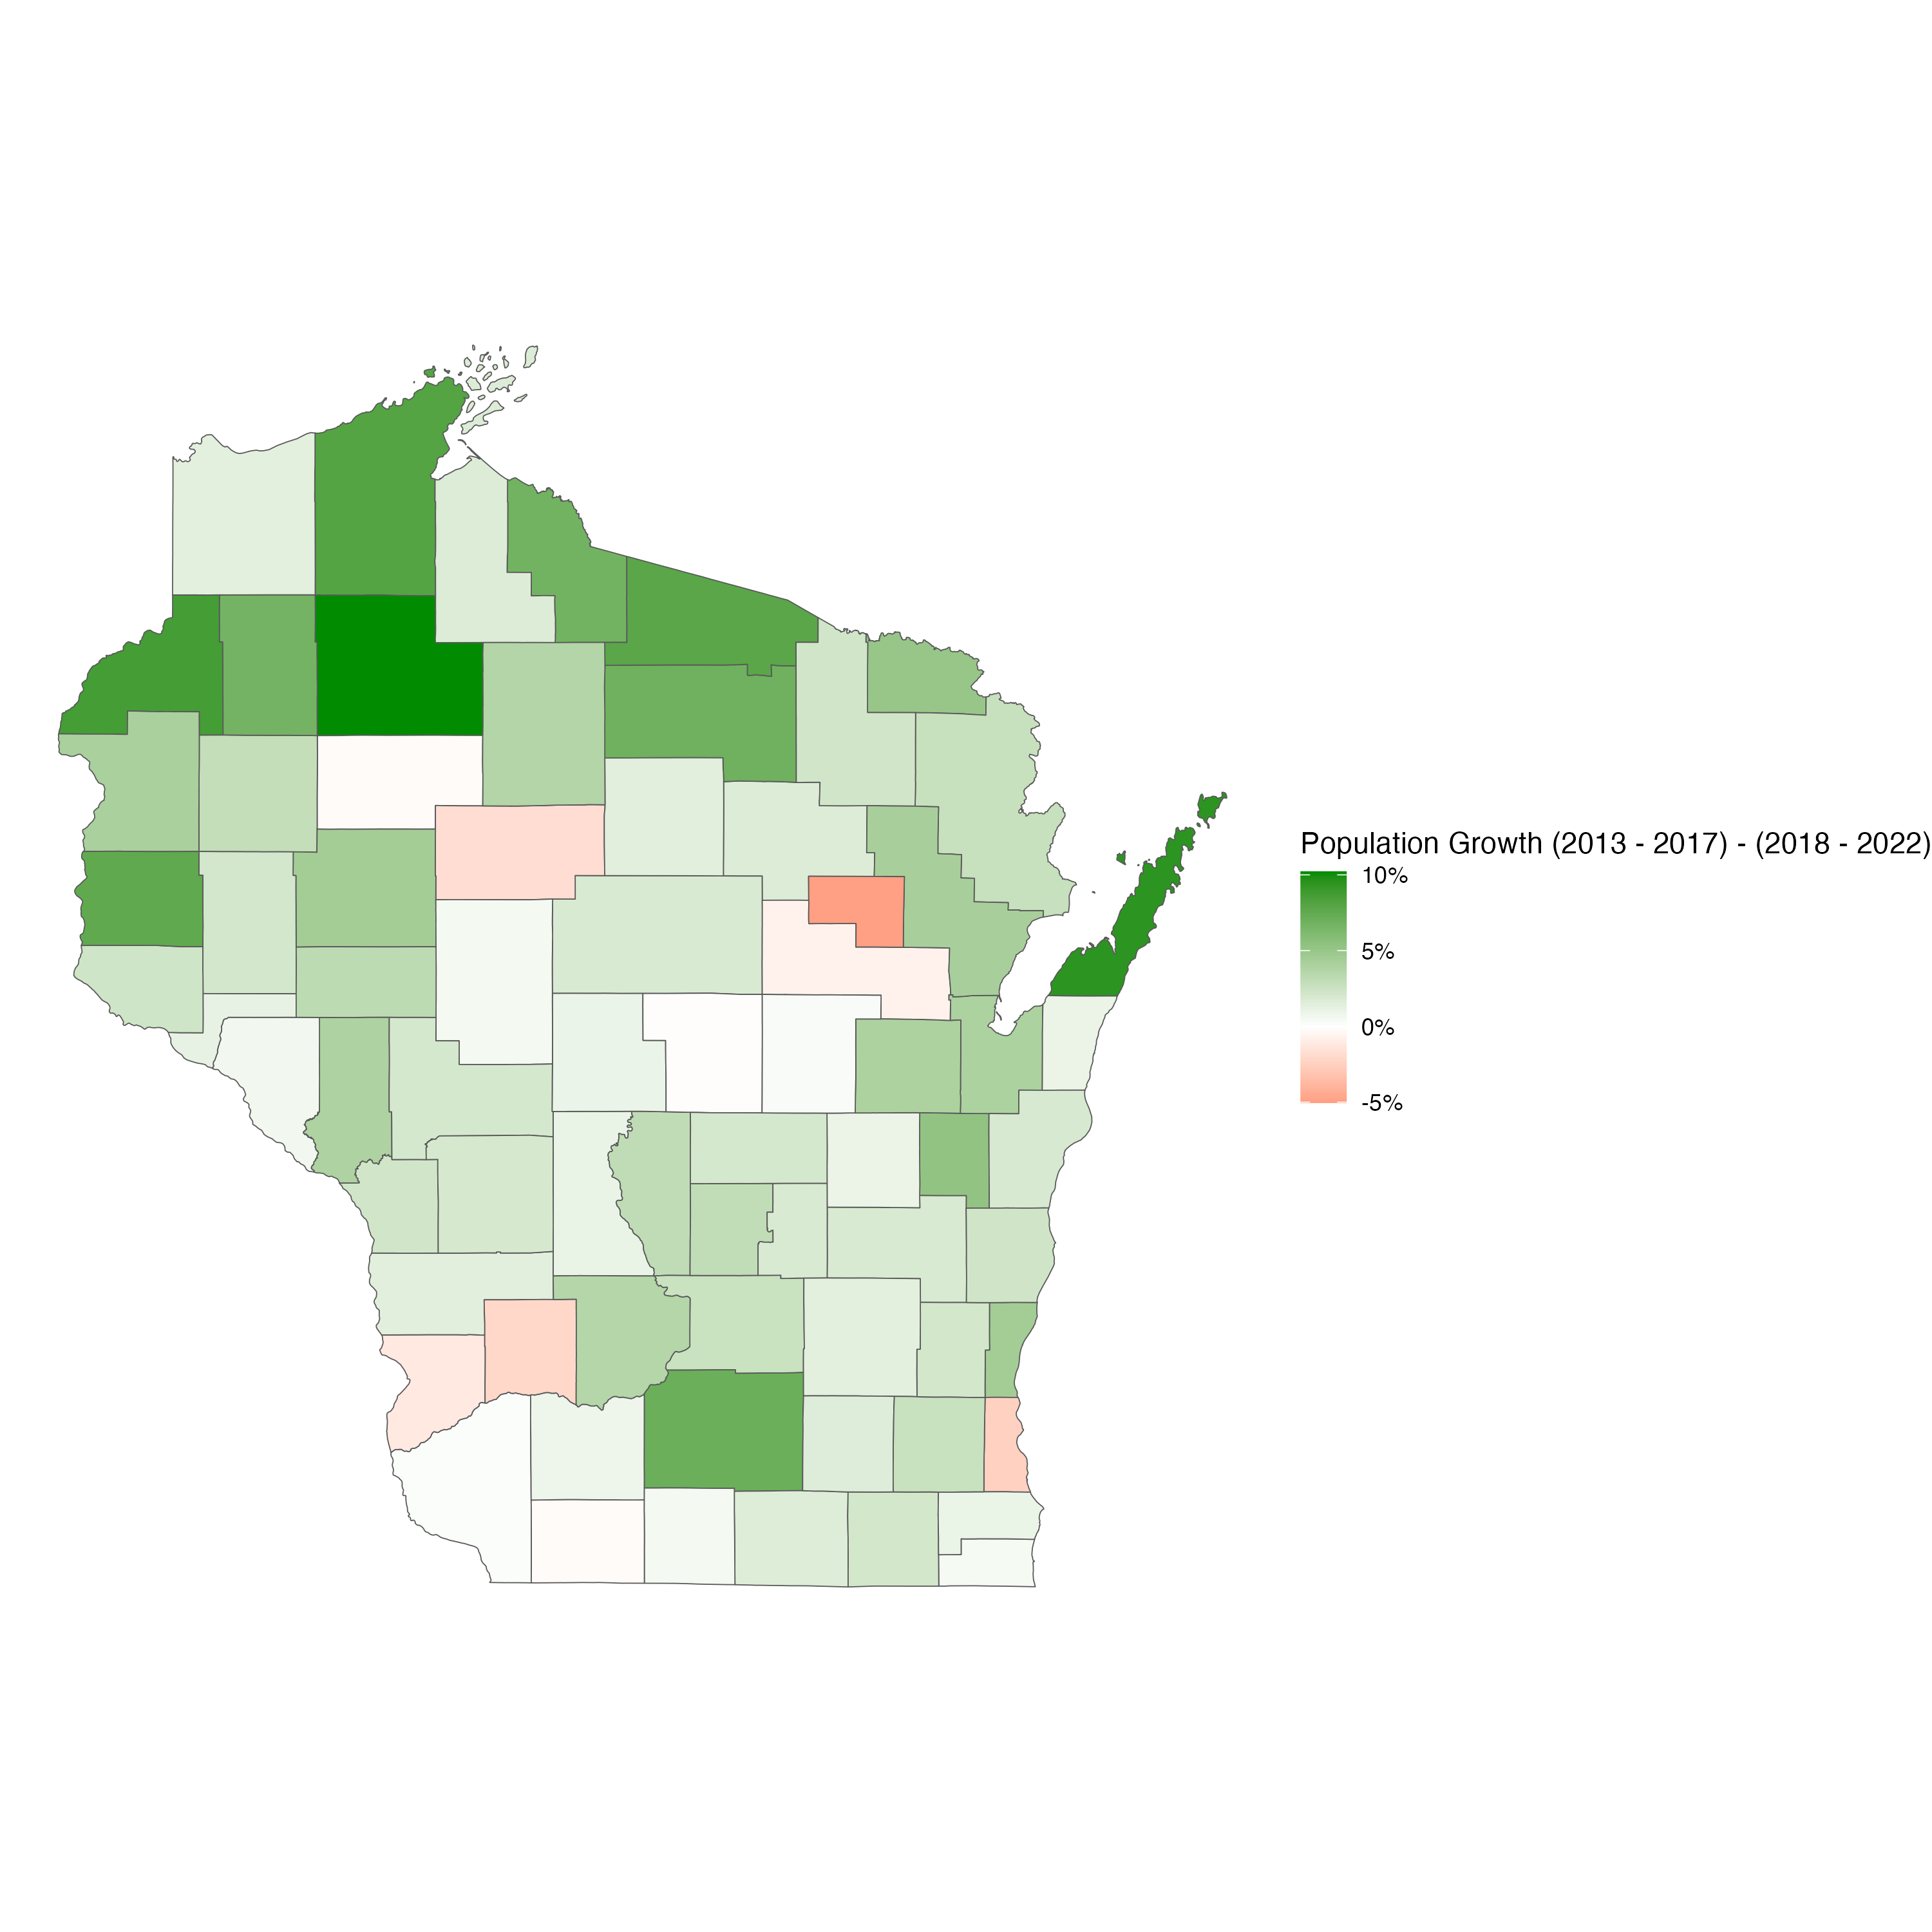
\includegraphics[width=0.9\textwidth]{plots/wi-growth.png}
    \caption{Wisconsin: County level population growth from the 2017 ACS to the 2022 ACS}
\end{figure}
\begin{figure}
   \centering
   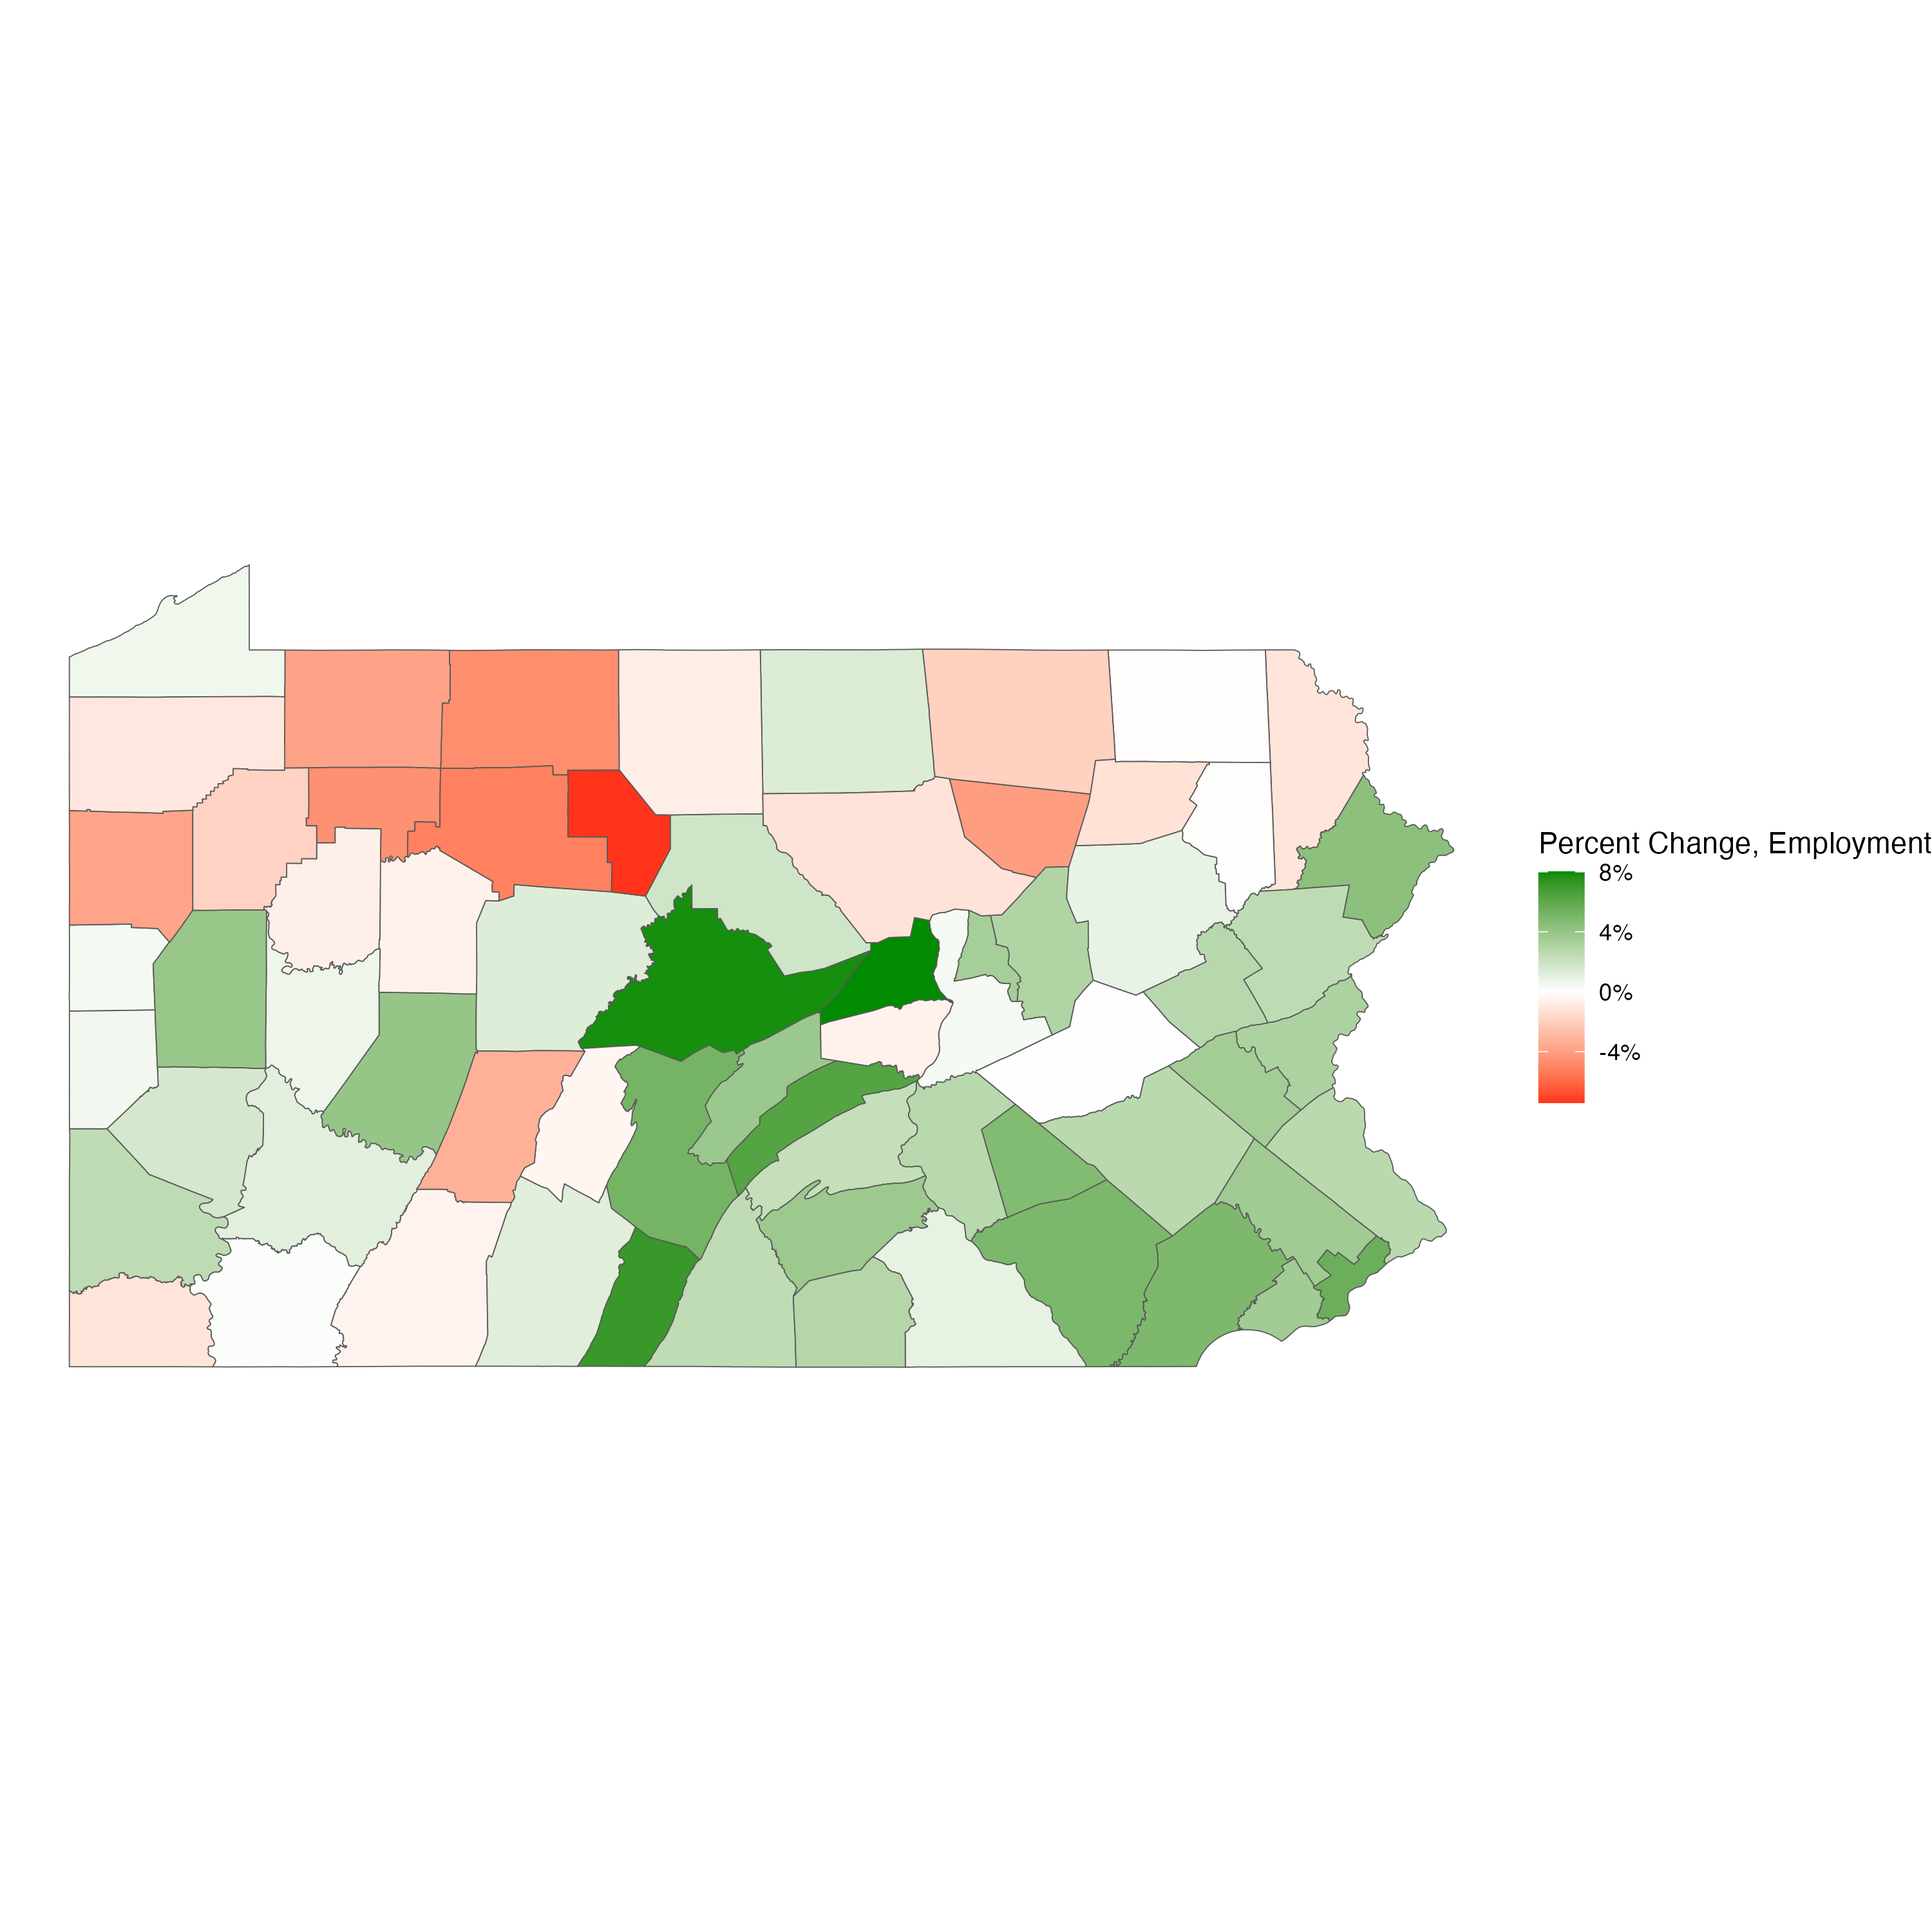
\includegraphics[width=0.9\textwidth]{plots/raw-employment-plot-pa.png}
   \caption{Pennsylvania: The percent change in the number of employed workers in each County from Trump's inauguration to February 2020, the Month before the pandemic hit}
\end{figure}
\begin{figure}
    \centering
    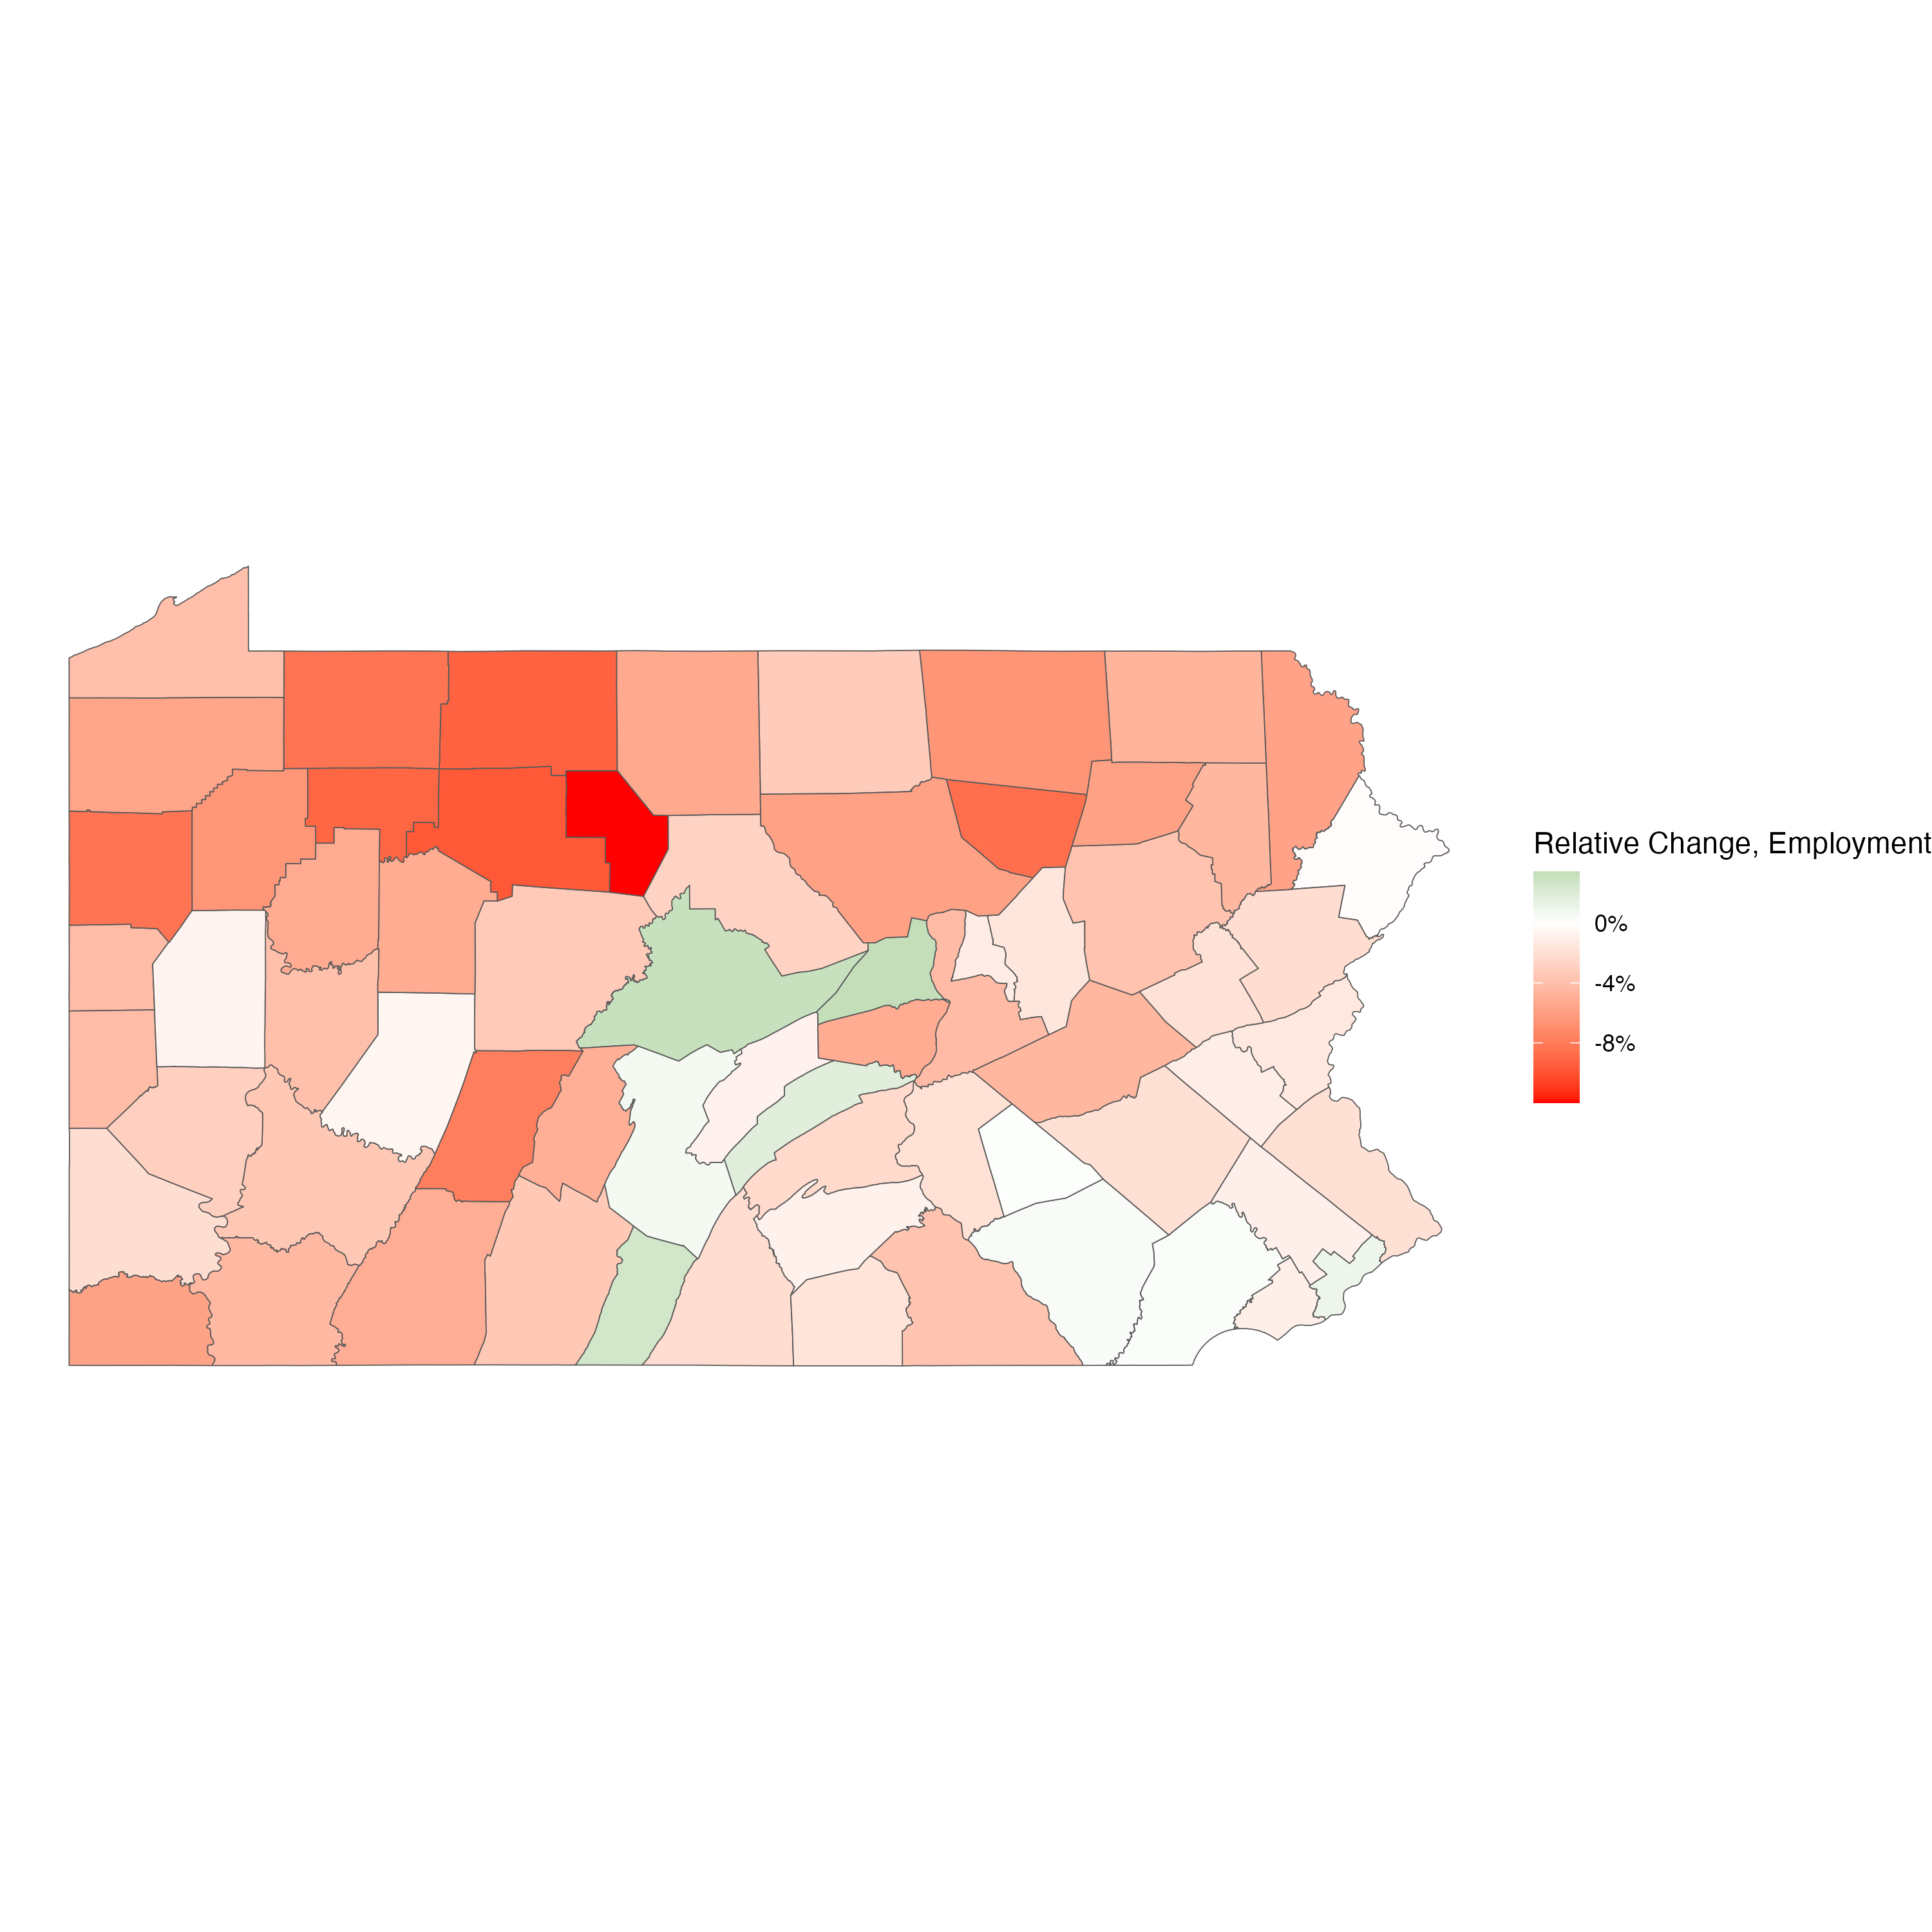
\includegraphics[width=0.9\textwidth]{plots/relative-employment-plot-pa.png}
    \caption{The percent change in the number of employed workers in each county in Pennsylvania minus the national percent change in the number of percent workers over the period from Trump's inauguration to February 2020}
\end{figure}
\begin{figure}
    \centering
    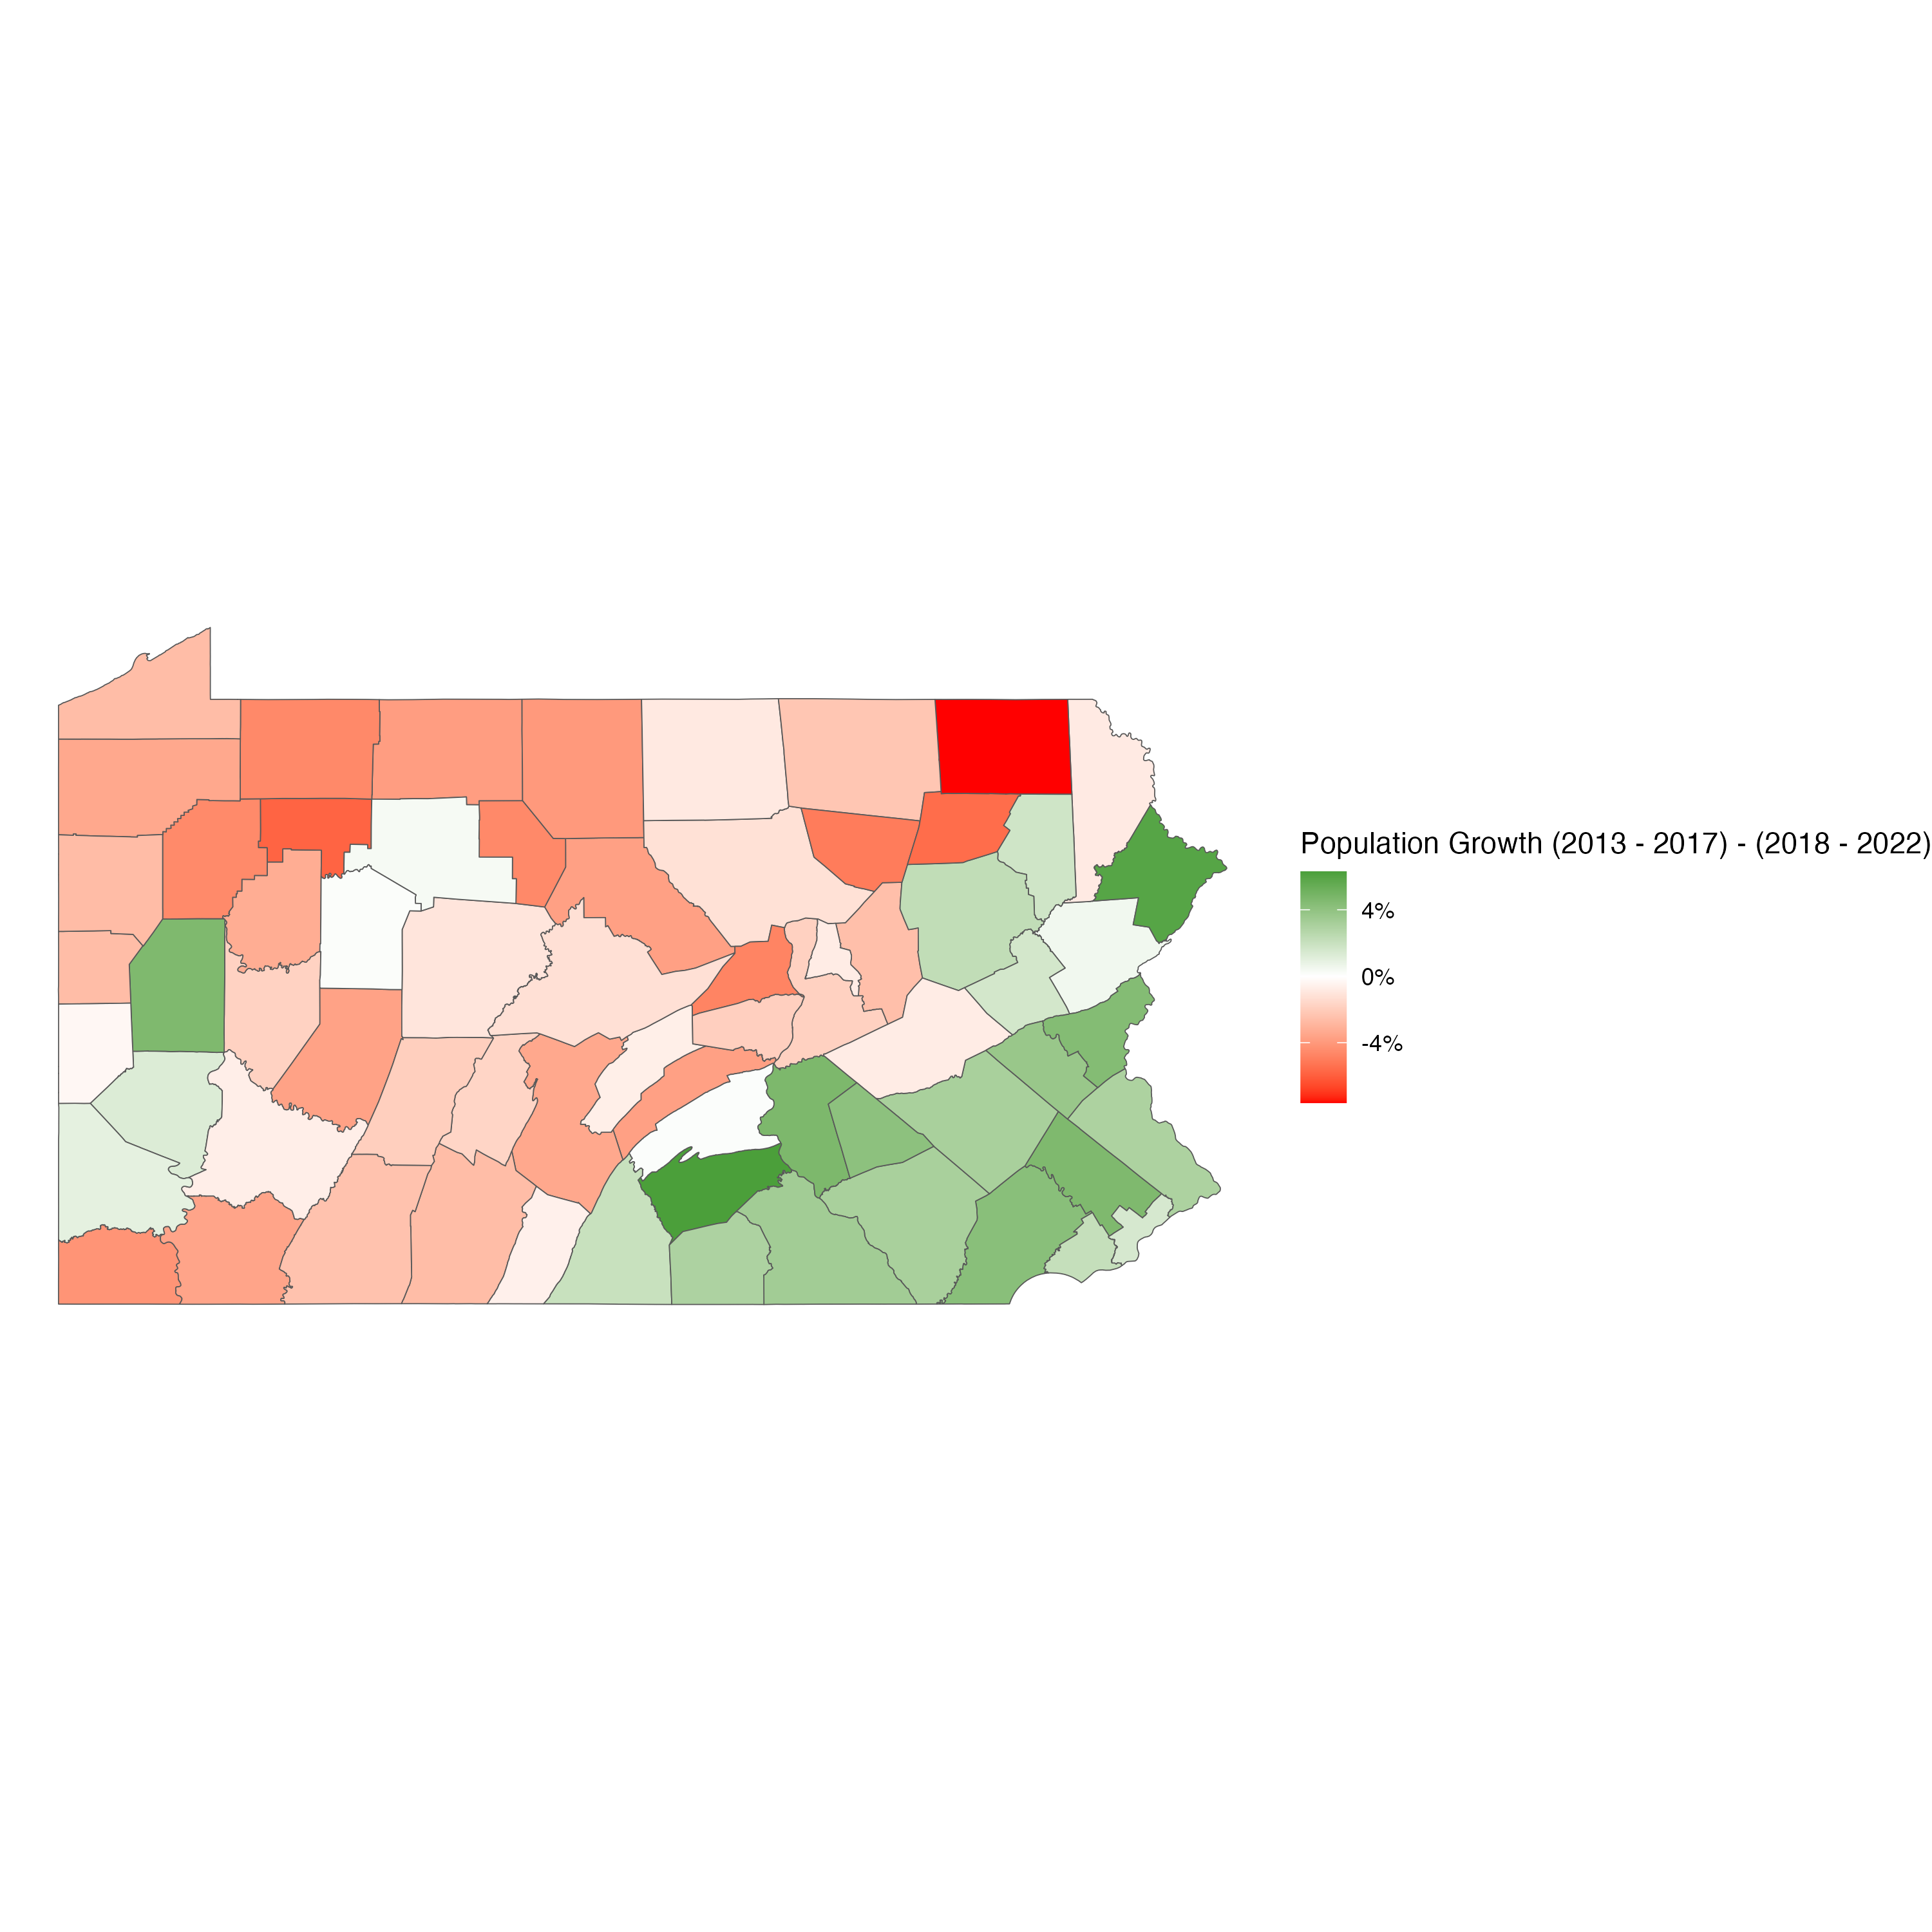
\includegraphics[width=0.9\textwidth]{plots/pa-growth.png}
    \caption{Pennsylvania: County level population growth from the 2017 ACS to the 2022 ACS}
\end{figure}
\begin{figure}
   \centering
   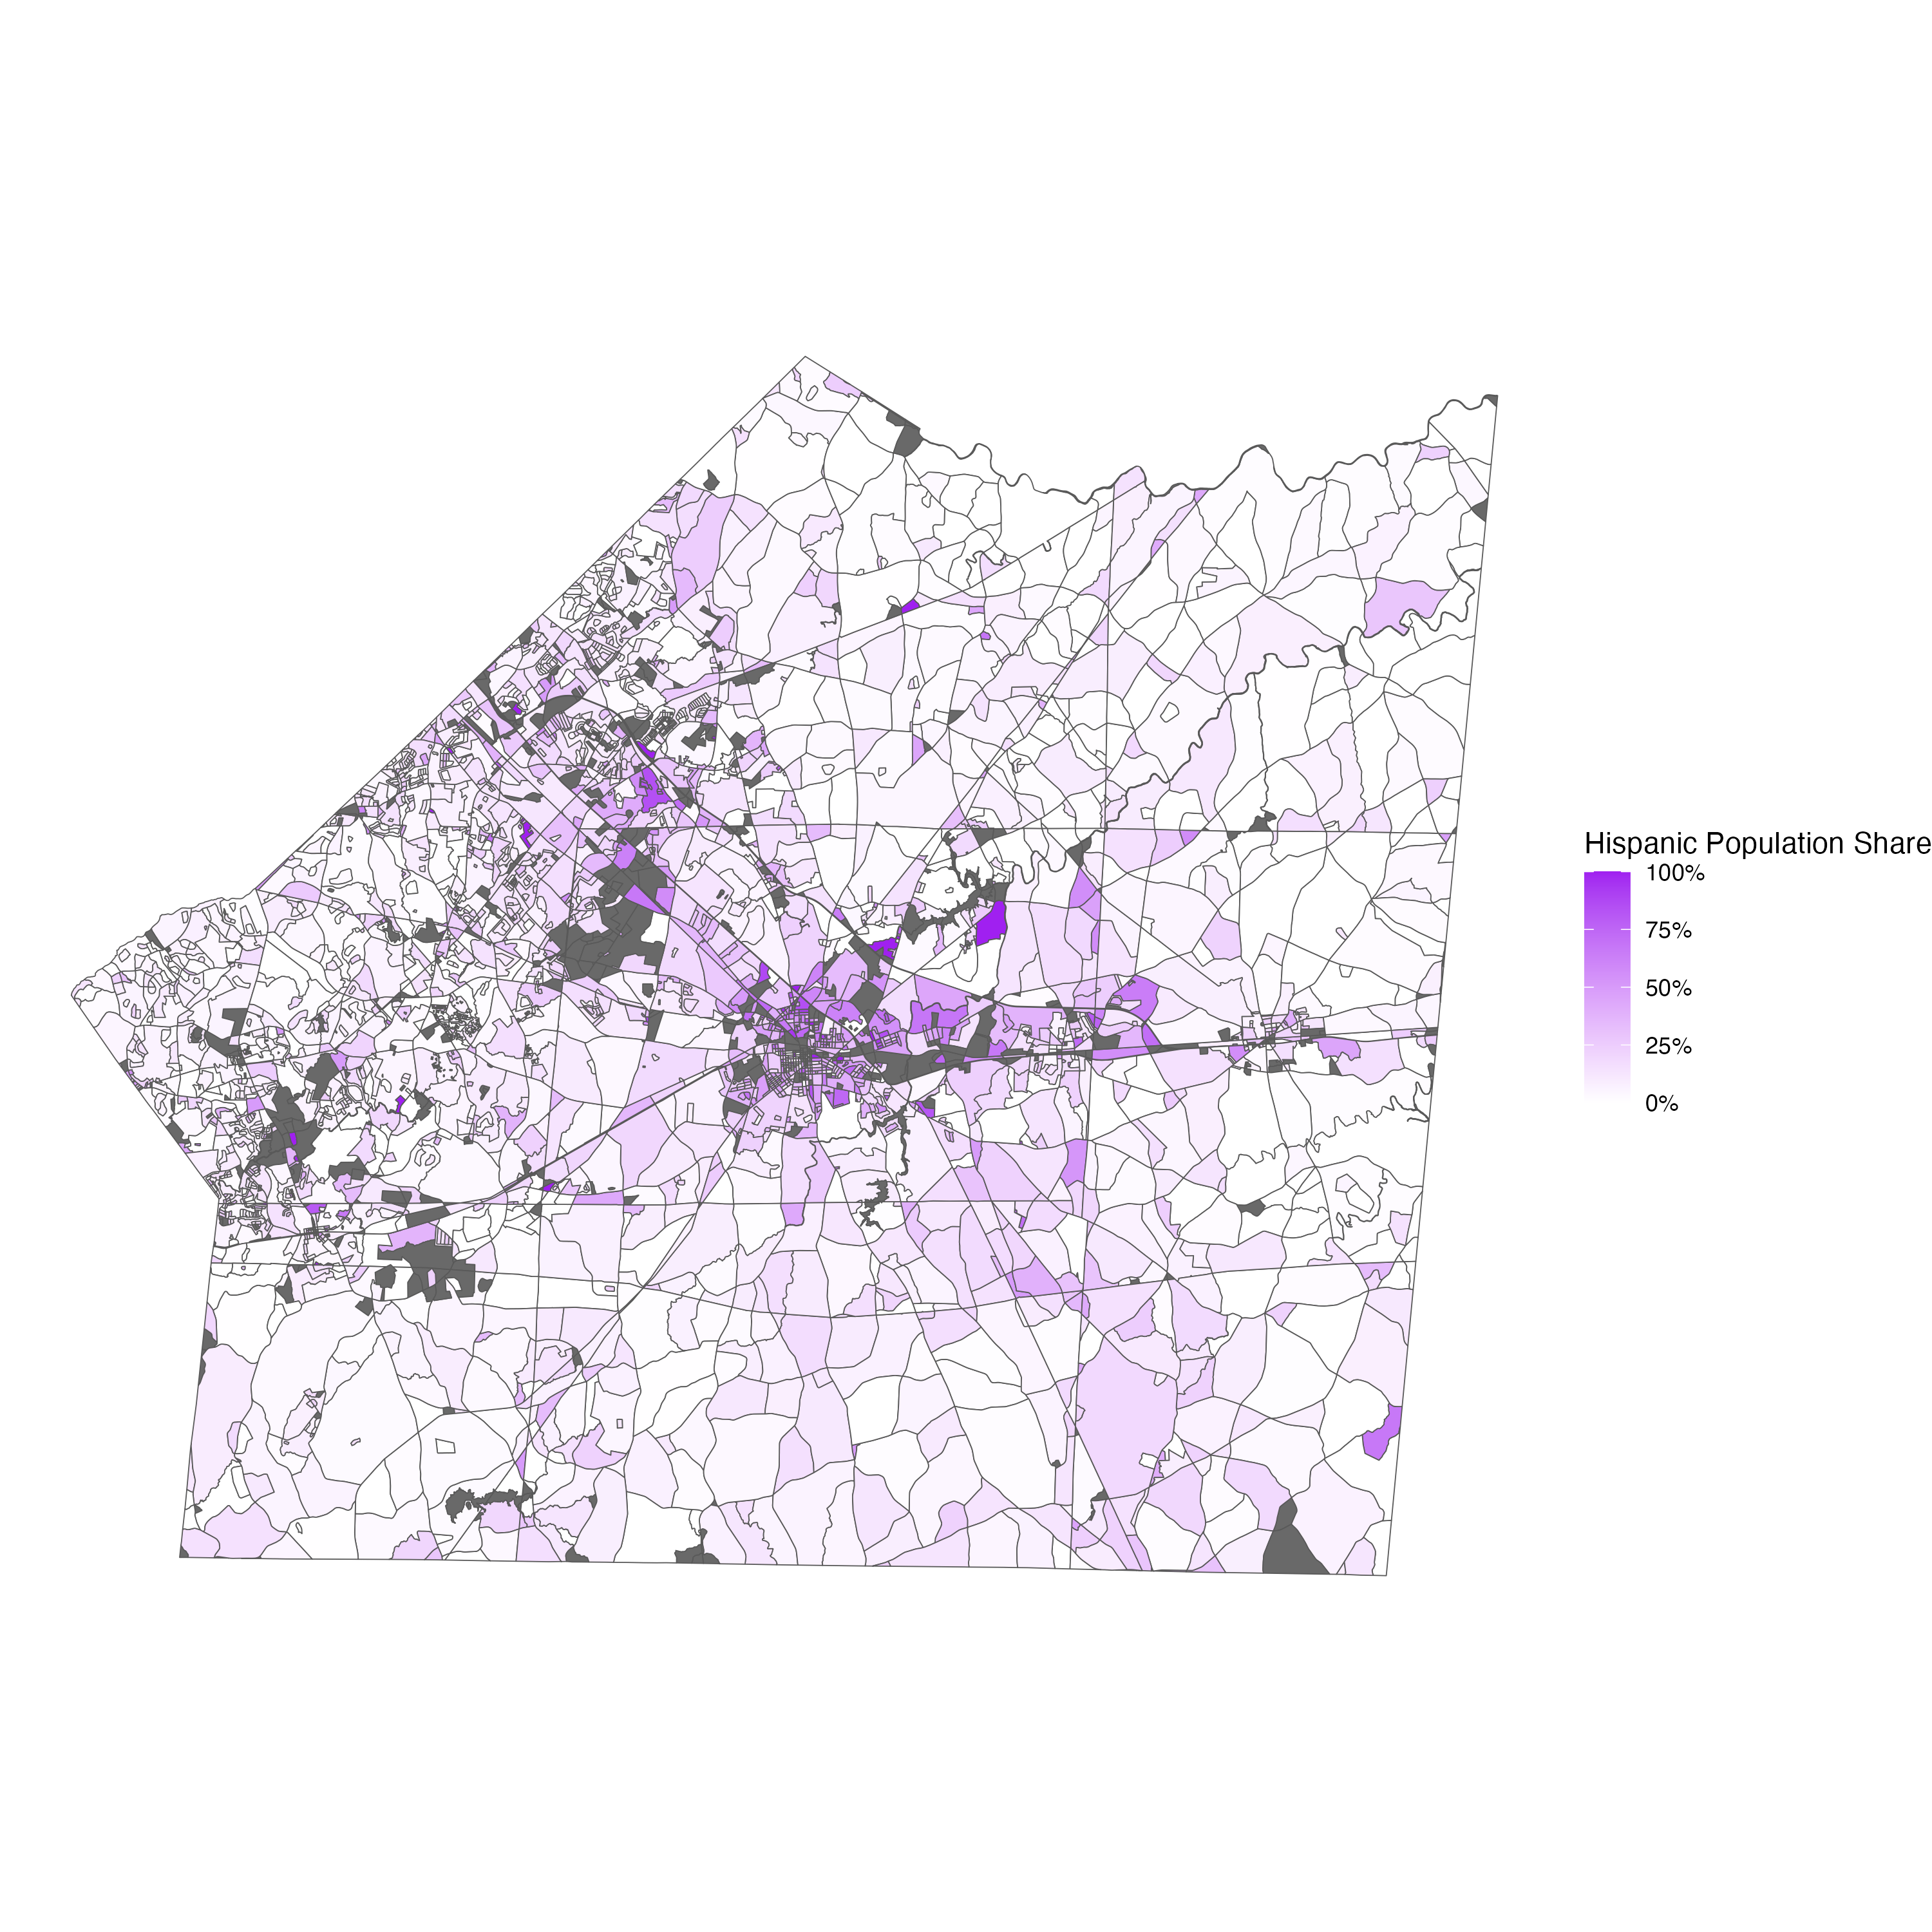
\includegraphics[width=0.9\textwidth]{plots/union_nc.png}
   \caption{2020 Census: Hispanic Population Share by block in Union County, NC}
\end{figure}
\end{document}
